\documentclass[aspectratio=169, 10pt]{beamer}

% =========================================================================
% MINIMALIST BEIGE & NAVY THEME (MARP / PROJECT PROPOSAL STYLE)
% Custom crafted to match the user's visual identity:
% Background: #F3EBE1 (Warm Cream Beige)
% Typography & Elements: #262E5B (Deep Indigo Navy)
% Signature: Right-edge vertical Navy bar with rounded inner corners
% =========================================================================

\usetheme{default}
\setbeamertemplate{navigation symbols}{}
\setbeamertemplate{headline}{}
\setbeamertemplate{footline}{}

\usepackage{fontspec}
% [SỬA LỖI 1] Segoe UI chỉ có trên Windows -> máy khác/Overleaf báo "font not found".
% Tự động dùng font dự phòng nếu không có Segoe UI.
\IfFontExistsTF{Segoe UI}{\setsansfont{Segoe UI}\setmainfont{Segoe UI}}{%
  \IfFontExistsTF{Carlito}{\setsansfont{Carlito}\setmainfont{Carlito}}{%
    \setsansfont{DejaVu Sans Condensed}\setmainfont{DejaVu Sans Condensed}}}

\usepackage{graphicx}
\usepackage{booktabs}
\usepackage{amsmath,amssymb}
\usepackage{xcolor}
\usepackage{tikz}
\usetikzlibrary{calc,positioning,shapes.geometric,arrows.meta}

% --- COLOR DEFINITIONS ---
\definecolor{bgBeige}{RGB}{243, 235, 225}    % #F3EBE1 - Warm Beige Canvas
\definecolor{navyMain}{RGB}{38, 46, 91}      % #262E5B - Deep Indigo Navy
\definecolor{navyMuted}{RGB}{85, 95, 140}    % Muted Navy for subtext/metadata
\definecolor{navyLight}{RGB}{228, 225, 235}  % Soft tinted fill
\definecolor{accentDark}{RGB}{185, 28, 28}   % Alert crimson

\setbeamercolor{background canvas}{bg=bgBeige}
\setbeamercolor{normal text}{fg=navyMain}
\setbeamercolor{structure}{fg=navyMain}

% Set margins so text never touches the right navy bar
\setbeamersize{text margin left=1.0cm, text margin right=1.8cm}

% --- SIGNATURE BACKGROUND WITH RIGHT NAVY ACCENT BAR ---
\setbeamertemplate{background}{
    \begin{tikzpicture}[remember picture,overlay]
        % Base Beige Canvas
        \fill[bgBeige] (current page.south west) rectangle (current page.north east);
        % Right vertical navy bar with 2 rounded inside corners (top-left & bottom-left)
        \fill[navyMain, rounded corners=16pt] 
            ($(current page.north east)+(-1.05cm, 0)$) rectangle ($(current page.south east)+(1.0cm, 0)$);
    \end{tikzpicture}
}

% --- CUSTOM SLIDE HEADER ---
\newcommand{\slideheader}[2]{%
    \vspace*{-0.15cm}%
    {\fontsize{7.5pt}{9pt}\selectfont \textbf{\color{navyMuted}\MakeUppercase{#1}}}\\[0.03cm]
    {\fontsize{13.5pt}{16pt}\selectfont \textbf{\color{navyMain}\MakeUppercase{#2}}}\\[0.08cm]
}

% --- CUSTOM FOOTER NUMBER ---
\newcommand{\slidenumber}[1]{%
    \begin{tikzpicture}[remember picture,overlay]
        \node[anchor=south east] at ($(current page.south east)+(-1.4cm, 0.35cm)$) {
            \textcolor{navyMuted}{\fontsize{8.5pt}{10pt}\selectfont \textbf{\insertframenumber}}
        };
        \node[anchor=south west] at ($(current page.south west)+(1.0cm, 0.35cm)$) {
            \textcolor{navyMuted}{\fontsize{7pt}{8pt}\selectfont \textit{Hands-On Data Visualization} -- Jack Dougherty \& Ilya Ilyankou}
        };
    \end{tikzpicture}%
}

% --- PILL BOX MACRO ---

\definecolor{boxBg}{RGB}{230, 221, 208}      % Tinted card bg #E6DDD0
\definecolor{accentRed}{RGB}{185, 28, 28}    % Alert crimson #B91C1C

\newcommand{\calloutbox}[3][\textwidth]{%
    \begin{tikzpicture}
        \node[
            fill=boxBg,
            draw=navyMain,
            line width=0.8pt,
            rounded corners=4pt,
            inner sep=5pt,
            text width=#1-14pt,
            align=left
        ] {
            {\fontsize{8.5pt}{10.5pt}\selectfont \textbf{\color{navyMain}#2}}\\[0.03cm]
            {\fontsize{7.5pt}{9.5pt}\selectfont \color{navyMain}#3}
        };
    \end{tikzpicture}%
}

\newcommand{\pillbox}[2][]{%
    \begin{tikzpicture}
        \node[
            draw=navyMain,
            rounded corners=10pt,
            line width=1.1pt,
            inner xsep=12pt,
            inner ysep=4pt,
            text=navyMain,
            #1
        ] {\textbf{#2}};
    \end{tikzpicture}%
}

% [SỬA LỖI 2] Thiếu file ảnh trong images/ -> lỗi "File not found" và dừng biên dịch.
% Nếu ảnh có thật: chèn bình thường. Nếu chưa có: vẽ khung giữ chỗ cùng kích thước.
\pgfkeys{/ph/.is family, /ph,
  width/.store in=\phw, height/.store in=\phh, .unknown/.code={}}
\let\origincludegraphics\includegraphics
\renewcommand{\includegraphics}[2][]{%
  \IfFileExists{#2}{\origincludegraphics[#1]{#2}}{%
    \begingroup
    \pgfkeys{/ph, width=\linewidth, height=0.4\textheight, #1}%
    \begin{tikzpicture}
      \node[draw=navyMuted, dashed, line width=0.7pt, fill=white!55!bgBeige, rounded corners=3pt,
            minimum width=\phw, minimum height={0.8*(\phh)}, text width={\phw-8pt}, align=center,
            font=\fontsize{6pt}{7.5pt}\selectfont, text=navyMuted]
        {\textbf{[Chèn ảnh]}\\\detokenize{#2}};
    \end{tikzpicture}%
    \endgroup}}


% Concise on-slide text; longer explanations stay in hidden Beamer notes.
\setbeameroption{hide notes}
\providecommand{\bodytext}{\fontsize{10pt}{13pt}\selectfont\raggedright}
\providecommand{\figcaption}[1]{{\fontsize{7.5pt}{9.5pt}\selectfont\color{navyMuted}#1\par}}
\providecommand{\takeaway}[1]{\vspace{0.18cm}{\fontsize{9.5pt}{12.5pt}\selectfont\bfseries #1\par}}
\providecommand{\briefdef}[2]{{\fontsize{10pt}{13pt}\selectfont\textbf{#1} #2\par}\vspace{0.20cm}}

\providecommand{\conceptcard}[3]{%
    \begin{tikzpicture}
    \node[fill=boxBg,draw=navyMain,line width=0.7pt,rounded corners=4pt,
      inner sep=8pt,align=left] {\parbox[t][3.45cm][t]{\dimexpr\linewidth-17pt\relax}{\raggedright%
      {\fontsize{10pt}{12.5pt}\selectfont\bfseries #1}\\[0.18cm]
      {\fontsize{9pt}{12pt}\selectfont #2}\\[0.18cm]
      {\fontsize{9pt}{12pt}\selectfont #3}
    }};
    \end{tikzpicture}%
}

\providecommand{\biasexample}[3]{%
\begin{tikzpicture}
\node[fill=boxBg,draw=navyMain,line width=0.7pt,rounded corners=4pt,
inner sep=8pt,text width=\dimexpr\linewidth-17pt\relax,
minimum height=2.55cm,align=left] {
{\fontsize{10pt}{12pt}\selectfont\bfseries #1}\\[0.12cm]
{\fontsize{8.5pt}{11pt}\selectfont\raggedright #2}\\[0.12cm]
{\fontsize{8.5pt}{11pt}\selectfont\color{navyMuted}#3}
};
\end{tikzpicture}%
}

\begin{document}

% ==================== SLIDE 1: TRANG TIÊU ĐỀ ====================


\begin{frame}[plain, c]


\begin{tikzpicture}[remember picture,overlay]
    
    % Main Title Block
    \node[anchor=west, text width=0.78\textwidth] at ($(current page.west)+(1.0cm, 0.4cm)$) {
        {\fontsize{32pt}{36pt}\selectfont \textbf{\color{navyMain} TRỰC QUAN HÓA}}\\[0.15cm]
        {\fontsize{32pt}{36pt}\selectfont \textbf{\color{navyMain} DỮ LIỆU}}\\[0.35cm]
        
        \pillbox{\fontsize{11pt}{13pt}\selectfont Kể chuyện Trực quan \& Nguyên lý Thiết kế}\\[0.4cm]
        
        {\small \color{navyMuted} Dựa trên tác phẩm: \textit{Hands-On Data Visualization} (Jack Dougherty \& Ilya Ilyankou)}
    };
    
    % Presenter info at bottom-left
    \node[anchor=south west] at ($(current page.south west)+(1.0cm, 0.9cm)$) {
        \textcolor{navyMain}{\fontsize{9.5pt}{11pt}\selectfont Thuyết trình bởi: \textbf{Nhóm 4 Thuyết Trình Viên}}
    };
\end{tikzpicture}
\end{frame}

% ==================== SLIDE 2: NỘI DUNG TRÌNH BÀY (OUR CONTENTS) ====================

\begin{frame}[plain, t]


\slideheader{Tổng quan bài báo cáo}{Nội Dung Trình Bày}

\vspace{0.2cm}
\begin{columns}[T]
\begin{column}{0.48\textwidth}
\begin{tikzpicture}
    \node[draw=navyMain, rounded corners=12pt, line width=1.1pt, inner xsep=14pt, inner ysep=8pt, minimum width=0.95\textwidth, text width=0.85\textwidth, align=left] {
        {\large \textbf{\color{navyMain} 01. Nền Tảng Dữ Liệu}}\\[3pt]
        \footnotesize \textcolor{navyMuted}{Thu thập, làm sạch \& so sánh có ý nghĩa (Ch. 3, 4, 5)}\\[2pt]
        \scriptsize \textbf{Người thuyết trình: Người 1}
    };
\end{tikzpicture}

\vspace{0.35cm}
\begin{tikzpicture}
    \node[draw=navyMain, rounded corners=12pt, line width=1.1pt, inner xsep=14pt, inner ysep=8pt, minimum width=0.95\textwidth, text width=0.85\textwidth, align=left] {
        {\large \textbf{\color{navyMain} 02. Thiết Kế Biểu Đồ}}\\[3pt]
        \footnotesize \textcolor{navyMuted}{Cấu trúc đồ thị, Zero-baseline \& phối màu (Ch. 6)}\\[2pt]
        \scriptsize \textbf{Người thuyết trình: Người 2}
    };
\end{tikzpicture}
\end{column}

\begin{column}{0.48\textwidth}
\begin{tikzpicture}
    \node[draw=navyMain, rounded corners=12pt, line width=1.1pt, inner xsep=14pt, inner ysep=8pt, minimum width=0.95\textwidth, text width=0.85\textwidth, align=left] {
        {\large \textbf{\color{navyMain} 03. Trực Quan Không Gian}}\\[3pt]
        \footnotesize \textcolor{navyMuted}{Bản đồ Choropleth, thang màu \& chuẩn hóa (Ch. 7)}\\[2pt]
        \scriptsize \textbf{Người thuyết trình: Người 3}
    };
\end{tikzpicture}

\vspace{0.35cm}
\begin{tikzpicture}
    \node[draw=navyMain, rounded corners=12pt, line width=1.1pt, inner xsep=14pt, inner ysep=8pt, minimum width=0.95\textwidth, text width=0.85\textwidth, align=left] {
        {\large \textbf{\color{navyMain} 04. Đạo Đức \& Kể Chuyện}}\\[3pt]
        \footnotesize \textcolor{navyMuted}{Nhận diện lừa dối, Cartogram \& Tell-Show-Why (Ch. 14, 15)}\\[2pt]
        \scriptsize \textbf{Người thuyết trình: Người 4}
    };
\end{tikzpicture}
\end{column}
\end{columns}

\slidenumber{02}
\end{frame}

% ==================== SLIDE 1: TRANG BÌA ====================
\begin{frame}[plain, c]
\begin{tikzpicture}[remember picture,overlay]
    \node[anchor=north west] at ($(current page.north west)+(1.0cm, -0.8cm)$) {
        \textcolor{navyMuted}{\fontsize{8.5pt}{10.5pt}\selectfont Tháng 10, 2026}
    };
    \node[anchor=west, text width=0.84\textwidth] at ($(current page.west)+(1.0cm, 0.3cm)$) {
        {\fontsize{13pt}{15pt}\selectfont \textbf{\color{navyMuted} PHẦN 1 • BÁO CÁO CHUYÊN ĐỀ}}\\[0.25cm]
        {\fontsize{29pt}{33pt}\selectfont \textbf{\color{navyMain} NỀN TẢNG DỮ LIỆU}}\\[0.12cm]
        {\fontsize{20pt}{24pt}\selectfont \textbf{\color{navyMain} THU THẬP, LÀM SẠCH \& CHUẨN HÓA}}\\[0.35cm]
        \pillbox{\fontsize{9.5pt}{11.5pt}\selectfont Từ Dữ Liệu Thô Đến Phép So Sánh Công Bằng (Chương 3, 4, 5)}\\[0.45cm]
        {\fontsize{8.5pt}{10.5pt}\selectfont \color{navyMuted} Thuyết trình: \textbf{Người 1} • Tác phẩm: \textit{Hands-On Data Visualization} (Jack Dougherty \& Ilya Ilyankou)}
    };
\end{tikzpicture}
\slidenumber{01}
\end{frame}
% ==================== SLIDE 4: TRIẾT LÝ DỮ LIỆU KHÔNG TRUNG LẬP ====================
\begin{frame}[plain, t]
\slideheader{Chương 3 • Triết Lý Cốt Lõi và Tìm Kiếm Dữ Liệu}{Dữ Liệu Không Bao Giờ Trung Lập}
\begin{columns}[T]
\begin{column}{0.54\textwidth}
{\fontsize{8pt}{10.2pt}\selectfont
\textbf{1. Sự ngộ nhận về ``Tính khách quan''}
\begin{itemize}\setlength{\itemsep}{1pt}
    \item Nhiều người lầm tưởng \textit{``con số không biết nói dối''}.
    \item Thực tế: Dữ liệu luôn do con người thu thập vì mục đích cụ thể.
    \item Chịu chi phối sâu sắc bởi bối cảnh lịch sử và cấu trúc quyền lực.
\end{itemize}

\vspace{0.06cm}
\textbf{2. 5 câu hỏi định hướng cốt lõi}
\begin{itemize}\setlength{\itemsep}{1pt}
    \item Mình muốn trả lời câu hỏi gì?
     \item Ai có thể đã thu thập?
 \item Dữ liệu chi tiết đến đâu?
\item Ai từng dùng dữ liệu này?
\item  Nếu chưa ai thu thập?
\end{itemize}
}
\end{column}
\begin{column}{0.42\textwidth}
\centering
\begin{tikzpicture}[scale=0.76]
    \fill[navyLight!50] (-3, 1.8) rectangle (3, 0);
    \fill[navyMain!15] (-3, 0) rectangle (3, -2.4);
    \draw[thick, navyMain] (-3, 0) -- (3, 0);
    \node[anchor=south east, font=\tiny\bfseries, color=navyMain] at (3, 0) {MẶT NƯỚC};
    \draw[draw=navyMain, fill=white, line width=1.1pt]
        (-1.0, 0) -- (-0.6, 1.4) -- (0.7, 1.5) -- (1.1, 0) --
        (1.9, -1.7) -- (-0.2, -2.3) -- (-1.9, -1.4) -- cycle;
    \node[font=\scriptsize\bfseries, color=navyMain, align=center] at (0.05, 0.7) {CON SỐ \& BẢNG BIỂU\\{\tiny (Phần nổi nhìn thấy)}};
    \node[font=\tiny\bfseries, color=navyMain, align=center] at (0, -0.5) {Mục đích thu thập};
    \node[font=\tiny\bfseries, color=navyMain, align=center] at (0, -1.0) {Cấu trúc quyền lực \& Bối cảnh};
    \node[font=\tiny\bfseries, color=accentRed, align=center] at (0, -1.6) {Những góc nhìn bị bỏ sót};
\end{tikzpicture}\\[0.05cm]
{\fontsize{6.5pt}{7.5pt}\selectfont \textcolor{navyMuted}{\textit{Sơ đồ Tảng băng trôi: Dữ liệu luôn có phần chìm chi phối.}}}
\end{column}
\end{columns}
\slidenumber{04}
\end{frame}
% ==================== SLIDE 8: PUBLIC VS PRIVATE ====================
\begin{frame}[plain, t]
\slideheader{Chương 3 • Pháp Lý \& Đạo Đức}{Dữ Liệu Công Khai vs. Riêng Tư}
{\fontsize{7.5pt}{9.2pt}\selectfont
\begin{center}
\begin{tabular}{p{0.17\textwidth} p{0.34\textwidth} p{0.37\textwidth}}
\toprule
\textbf{\color{navyMain} Khía cạnh} & \textbf{\color{navyMain} Khu vực Tư nhân} & \textbf{\color{navyMain} Khu vực Công} \\
\midrule
\textbf{Thực trạng thu thập} & \textbf{Chủ nghĩa tư bản giám sát}: Google, Amazon, Meta. & Dữ liệu công dân; công chúng dùng \textbf{Đạo luật Tự do Thông tin} / Sunshine Laws để giám sát. \\
\midrule
\textbf{Dữ liệu cấm công khai cá nhân} & Phụ thuộc chính sách nội bộ và đạo luật người tiêu dùng. & • \textbf{HIPAA:} Bảo mật hồ sơ bệnh án.\newline
• \textbf{FERPA:} Bảo mật điểm học tập.\newline
$\rightarrow$ \textit{Bắt buộc ẩn danh hóa \& gom cụm.} \\
\midrule
\textbf{Dữ liệu cá nhân công khai vì cộng đồng} & Dữ liệu di chuyển tổng hợp. & 1. Đóng góp tài chính bầu cử.\newline
2. Hồ sơ sở hữu và giá trị bất động sản.\newline
3. Lương lãnh đạo quỹ phi lợi nhuận.\newline
4. Hồ sơ cảnh sát dùng vũ lực. \\
\bottomrule
\end{tabular}
\end{center}
}
\slidenumber{08}
\end{frame}

% ==================== SLIDE 9: MASKING & AGGREGATING ====================
\begin{frame}[plain, t]
\slideheader{Chương 3 • Đạo Đức Dữ Liệu}{Bảo Vệ Danh Tính: Làm Mờ \& Tổng Hợp}
\begin{columns}[T]
\begin{column}{0.52\textwidth}
{\fontsize{8.2pt}{10.5pt}\selectfont
Để đảm bảo \textbf{tính minh bạch, độ tin cậy và khả năng tái lập }, hãy rèn luyện 3 thói quen ngay khi tải file:

\vspace{0.12cm}
\textbf{1. Đặt tên file có ý nghĩa}
\begin{itemize}\setlength{\itemsep}{1.5pt}
    \item \textcolor{accentRed}{\textbf{Tránh:}} \texttt{data.csv}, \texttt{download.xlsx}, \texttt{file(1).csv}.
    \item \textbf{Chuẩn:} Nguồn + Chủ đề + Ngày \texttt{YYYY-MM-DD} (chữ thường, gạch nối):\\ \texttt{eurostat-co2-emissions-2020-05-01.xlsx}.
\end{itemize}

\vspace{0.12cm}
\textbf{2. Tạo tab \texttt{notes} riêng biệt bên trong bảng tính}
\begin{itemize}\setlength{\itemsep}{1.5pt}
    \item Ghi rõ cơ quan ban hành, URL tải, định nghĩa nhãn viết tắt, người tải và ngày cập nhật.
\end{itemize}

\vspace{0.12cm}
\textbf{3. Tạo tab \texttt{backup} bất khả xâm phạm}
\begin{itemize}\setlength{\itemsep}{1.5pt}
    \item Giữ nguyên dữ liệu gốc, thao tác làm sạch ở tab \texttt{data}.
\end{itemize}
}
\end{column}
\begin{column}{0.44\textwidth}
\centering
\begin{tikzpicture}[scale=0.85]
    \node[draw=navyMain, fill=white, rounded corners=4pt, align=center, font=\scriptsize\bfseries] (raw) at (0, 2.3) {DỮ LIỆU GỐC NGUY HIỂM\\{\tiny 1234 Main St | Aggravated Assault}};
    \node[draw=navyMain, fill=boxBg, rounded corners=4pt, align=center, font=\scriptsize\bfseries, text width=2.3cm] (mask) at (-1.55, 0.45) {1. LÀM MỜ\\(MASKING)\\{\tiny Ẩn ký tự cuối địa chỉ}\\{\tiny \textbf{1XXX Main St}}};
    \node[draw=navyMain, fill=boxBg, rounded corners=4pt, align=center, font=\scriptsize\bfseries, text width=2.3cm] (agg) at (1.55, 0.45) {2. TỔNG HỢP\\(AGGREGATING)\\{\tiny Gom theo khu phố/Tract}\\{\tiny \textbf{East Side: 13 vụ}}};
    \draw[-{Latex[length=2mm]}, line width=1.1pt, navyMain] (raw) -- (mask);
    \draw[-{Latex[length=2mm]}, line width=1.1pt, navyMain] (raw) -- (agg);
    \node[draw=navyMain, fill=navyLight, rounded corners=4pt, align=center, font=\tiny\bfseries, text width=4.2cm] (res) at (0, -1.25) {Vừa bảo vệ danh tính nạn nhân,\\vừa làm rõ xu hướng địa bàn phục vụ hoạch định};
    \draw[-{Latex[length=1.5mm]}, line width=0.8pt, navyMain] (mask) -- (res);
    \draw[-{Latex[length=1.5mm]}, line width=0.8pt, navyMain] (agg) -- (res);
\end{tikzpicture}
\end{column}
\end{columns}
\slidenumber{09}
\end{frame}
% ==================== SLIDE 11: BAD DATA ====================
\begin{frame}[plain, t]
\slideheader{Chương 3 • Nhận Diện Dữ Liệu Xấu}{4 Dấu Hiệu Dữ Liệu Lỗi Kinh Điển}
\begin{columns}[T]
\begin{column}{0.48\textwidth}
\calloutbox[\linewidth]{1. Missing Values Nhập Sai}{
    Ô trống (\texttt{null/blank}) có ý nghĩa khác số \texttt{0}.\\[0.05cm]
    \textbf{Cảnh báo:} Người nhập điền \texttt{0}, \texttt{-1}, \texttt{-999} để báo khuyết làm sai lệch hoàn toàn hàm \texttt{SUM}, \texttt{AVERAGE}!
}
\vspace{0.15cm}
\calloutbox[\linewidth]{2. Mất Số 0 Dẫn Đầu (Leading Zeros)}{
    Xảy ra khi phần mềm tự ép kiểu Text sang Number.\\[0.05cm]
    \textbf{Hậu quả:} Mã Zip \texttt{06106} bị biến thành \texttt{6106}. Mã FIPS hạt LA \texttt{037} biến thành \texttt{37} (nhầm sang bang Bắc Carolina)!
}
\end{column}
\begin{column}{0.48\textwidth}
\calloutbox[\linewidth]{3. Chạm Giới Hạn Dòng Của Phần Mềm}{
    Nếu dữ liệu dừng ở dòng thứ \textbf{65.536} (giới hạn Excel \texttt{.xls} cũ) $\rightarrow$ Dữ liệu đã bị cắt cụt!\\[0.05cm]
    \textbf{Thực tế:} Y tế Anh từng mất hàng ngàn mẫu xét nghiệm Covid-19 vì lỗi này.
}
\vspace{0.15cm}
\calloutbox[\linewidth]{4. Bất Nhất Định Dạng Ngày Tháng}{
    Nhầm giữa chuẩn Mỹ \texttt{MM/DD/YYYY} và Quốc tế \texttt{DD/MM/YYYY}.\\[0.05cm]
    Xuất hiện ngày mặc định hệ thống (\texttt{1/1/1900}, \texttt{1970}) hoặc số thứ tự nội bộ Excel (\texttt{43891}).
}
\end{column}
\end{columns}
\slidenumber{11}
\end{frame}

% ==================== SLIDE 12: GEOCODING ====================
\begin{frame}[plain, t]
\slideheader{Chương 3 • Nhận Diện Dữ Liệu Xấu}{Ảo Giác Địa Lý: Bẫy Geocoding Sai Lệch}
\begin{columns}[T]
\begin{column}{0.52\textwidth}
{\fontsize{8.2pt}{10.5pt}\selectfont
Khi chuyển đổi địa chỉ IP hoặc tọa độ thành điểm bản đồ, thuật toán Geocoding tự động có thể sinh ra bẫy chết người:

\vspace{0.15cm}
\textbf{1. Trang trại Bắc Kansas}
\begin{itemize}\setlength{\itemsep}{2pt}
    \item Một bản đồ từng chỉ ra cư dân vùng nông thôn Bắc Kansas xem web người lớn nhiều nhất nước Mỹ.
    \item \textbf{Sự thật:} Hàng triệu IP ẩn danh (VPN) không xác định vị trí bị tự động gán vào \textbf{tâm địa lý của lục địa Mỹ} (tình cờ trúng nông trại này).
\end{itemize}

\vspace{0.15cm}
\textbf{2. Đảo ảo ``Null Island'' $(0, 0)$}
\begin{itemize}\setlength{\itemsep}{2pt}
    \item Dữ liệu lỗi tọa độ bị gán về giao điểm Xích đạo và Kinh tuyến gốc giữa Đại Tây Dương (thực chất chỉ là một phao đo thời tiết).
\end{itemize}
}
\end{column}
\begin{column}{0.44\textwidth}
\centering
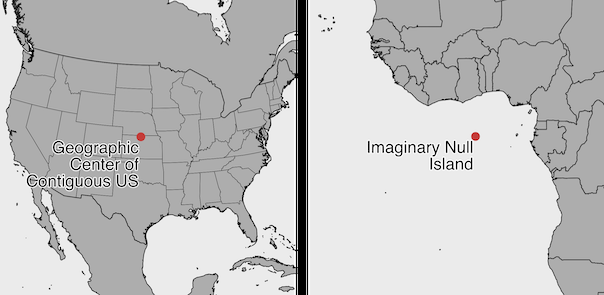
\includegraphics[width=\linewidth, height=0.52\textheight, keepaspectratio]{images/fig_3_4_null_island.png}\\[0.15cm]
{\fontsize{6.8pt}{8pt}\selectfont \textcolor{navyMuted}{\textit{Hình 3.4: Bẫy tâm địa lý Kansas (trái) \& Null Island tọa độ (0,0) (phải).}}}
\end{column}
\end{columns}
\slidenumber{12}
\end{frame}

% ==================== SLIDE 15: DỮ LIỆU THÔ ====================
\begin{frame}[plain, t]
\slideheader{Chương 4 • Dữ Liệu Thô, Làm Sạch}{Thực Trạng Phũ Phàng Của Bảng Dữ Liệu Thô}
\begin{columns}[T]
\begin{column}{0.52\textwidth}
{\fontsize{8.2pt}{10.5pt}\selectfont
\textbf{1. Trùng lặp \& Khoảng trắng thừa (Whitespaces)}
\begin{itemize}\setlength{\itemsep}{2pt}
    \item Khoảng trắng vô hình ở cuối chuỗi (\texttt{"Brazil "} vs \texttt{"Brazil"}) khiến máy tính coi đây là 2 quốc gia khác nhau khi gom nhóm.
\end{itemize}

\vspace{0.12cm}
\textbf{2. Tách đơn vị đo khỏi cột số}
\begin{itemize}\setlength{\itemsep}{2pt}
    \item Xóa bỏ ký hiệu \$, dấu phẩy, \texttt{kg}, \% (\texttt{282,805a} $\rightarrow$ \texttt{282805}) để đưa văn bản (căn trái) về số thực thụ (căn phải).
\end{itemize}

\vspace{0.12cm}
\textbf{3. Cẩn trọng khi Tìm \& Thay thế (Find \& Replace)}
\begin{itemize}\setlength{\itemsep}{2pt}
    \item \textbf{Bài toán:} 169 thị trấn Connecticut thừa chữ \texttt{"town"} (\texttt{Hartford town}, \texttt{Newtown town}).
    \item \textcolor{accentRed}{\textbf{Bẫy:}} Thay \texttt{"town"} $\rightarrow$ \texttt{Newtown} bị biến thành \texttt{New}!
    \item \textbf{Chuẩn:} Phải tìm chính xác chuỗi \textbf{\texttt{" town"} (có dấu cách phía trước)}.
\end{itemize}
}
\end{column}
\begin{column}{0.44\textwidth}
\centering
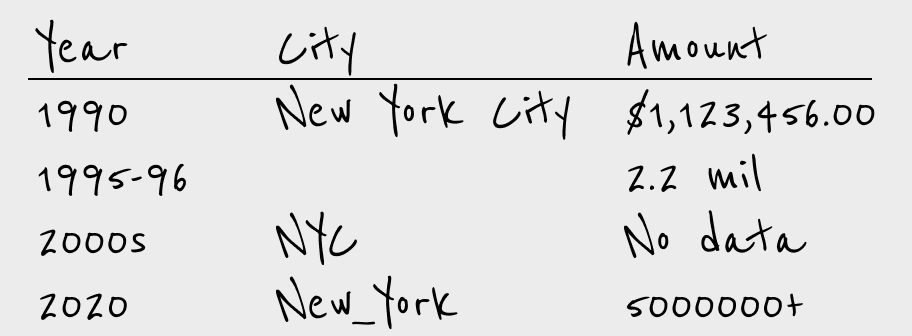
\includegraphics[width=\linewidth, height=0.52\textheight, keepaspectratio]{images/fig_4_1_messy_data.png}\\[0.15cm]
{\fontsize{6.8pt}{8pt}\selectfont \textcolor{navyMuted}{\textit{Hình 4.1: Bản phác thảo các lỗi định dạng kinh điển của dữ liệu thô.}}}
\end{column}
\end{columns}
\slidenumber{15}
\end{frame}
% ==================== SLIDE 17: TRANSPOSE, SPLIT & COMBINE ====================
\begin{frame}[plain, t]
\slideheader{Chương 4 • Kỹ Thuật Làm Sạch}{Tái Cấu Trúc Bảng: Transpose, Split \& Combine}
\begin{columns}[T]
\begin{column}{0.48\textwidth}
\calloutbox[\linewidth]{1. Xoay Trục Dữ Liệu: Transpose (Hàng $\leftrightarrow$ Cột)}{
    \textbf{Mâu thuẫn góc nhìn:}
    \begin{itemize}\setlength{\itemsep}{2pt}
        \item Khi trình bày \textbf{Bảng (Table)} cho người đọc: Thời gian xếp \textbf{nằm ngang} theo cột (\texttt{2000 | 2010 | 2020}).
        \item Khi vẽ \textbf{Biểu đồ đường}: Phần mềm yêu cầu thời gian phải chạy \textbf{thẳng đứng} theo cột đầu tiên từ trên xuống dưới.
    \end{itemize}
    $\rightarrow$ Kỹ thuật \textbf{Transpose} giúp đảo ngược ma trận Hàng $\leftrightarrow$ Cột tức thời mà không cần nhập lại dữ liệu.
}
\end{column}
\begin{column}{0.48\textwidth}
\calloutbox[\linewidth]{2. Tách Cột \& Gộp Cột }{
    \textbf{Tách cột:}
    \begin{itemize}\setlength{\itemsep}{1.5pt}
        \item Khi nhiều thực thể bị nhét chung vào 1 ô:
        \item \texttt{300 Summit St, Hartford CT--06106}
        \item Dùng dấu phân cách (\texttt{,}, khoảng trắng, \texttt{--}) tách thành 4 cột riêng: \texttt{Street | City | State | Zip}.
    \end{itemize}
    \vspace{0.08cm}
    \textbf{Gộp cột :}
    \begin{itemize}\setlength{\itemsep}{1.5pt}
        \item Ngược lại, khi nạp vào công cụ bản đồ, nối các cột địa chỉ rời rạc thành một chuỗi duy nhất có dấu phẩy phân cách.
    \end{itemize}
}
\end{column}
\end{columns}
\slidenumber{17}
\end{frame}

% ==================== SLIDE 18: CLUSTERING ====================
\begin{frame}[plain, t]
\slideheader{Chương 4 • Kỹ Thuật Làm Sạch}{Gom Cụm Chuẩn Hóa Tên Gọi}
\begin{columns}[T]
\begin{column}{0.51\textwidth}
{\fontsize{8.2pt}{10.5pt}\selectfont
\textbf{Thực tế dữ liệu viện trợ Mỹ:}
\begin{itemize}\setlength{\itemsep}{2pt}
    \item Chỉ riêng 2 quốc gia Triều Tiên và Hàn Quốc nhưng xuất hiện tới \textbf{26 cách viết khác nhau}:
    \texttt{Korea, N}, \texttt{Korea-North}, \texttt{SouthKorea}, \texttt{So Korea}, \texttt{Korea, South}...
    \item Cơ quan tài trợ sai chính tả: \texttt{Dept of Agriculture}, \texttt{Department of Argic}...
\end{itemize}

\vspace{0.12cm}
\textbf{Thuật toán Gom cụm thông minh:}
\begin{itemize}\setlength{\itemsep}{2pt}
    \item \textbf{Key Collision:} Chuẩn hóa chữ hoa/thường, xóa dấu câu, sắp xếp lại từ khóa. Tốc độ rất cao, quét tập dữ liệu lớn.
    \item \textbf{Nearest Neighbor:} Tính khoảng cách chỉnh sửa giữa các chuỗi để bắt các lỗi chính tả tinh vi.
\end{itemize}
}
\end{column}
\begin{column}{0.45\textwidth}
\centering
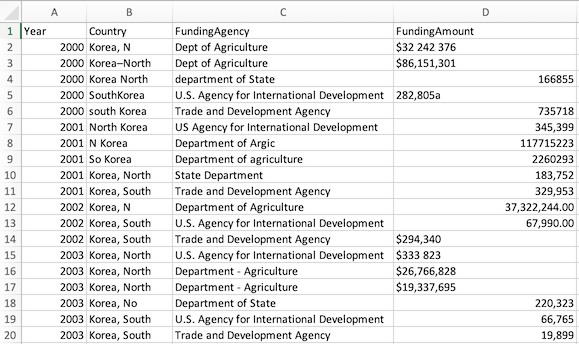
\includegraphics[width=\linewidth, height=0.25\textheight, keepaspectratio]{images/fig_4_11_korea_raw.png}\\[0.1cm]
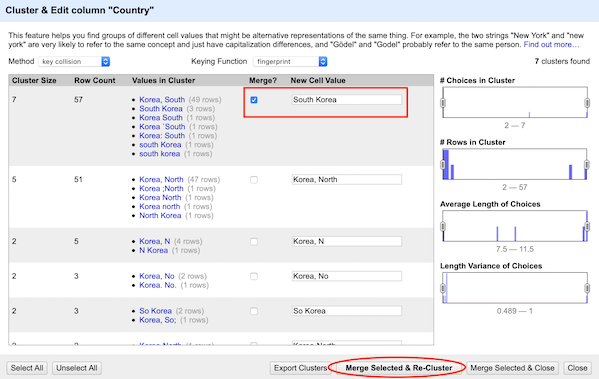
\includegraphics[width=\linewidth, height=0.26\textheight, keepaspectratio]{images/fig_4_18_korea_cluster.png}\\[0.1cm]
{\fontsize{6.5pt}{7.8pt}\selectfont \textcolor{navyMuted}{\textit{Hình 4.11: Dữ liệu thô lộn xộn \& Hình 4.18: Giao diện gom cụm về 1 tên.}}}
\end{column}
\end{columns}
\slidenumber{18}
\end{frame}

% ==================== SLIDE 19: CHUYỂN TIẾP CHƯƠNG 5 ====================

% ==================== SLIDE 20: MEAN VS. MEDIAN ====================
\begin{frame}[plain, t]
\slideheader{Chương 5 • Ngôn Từ Chuẩn Xác}{Trung Bình (Mean) vs. Trung Vị (Median)}
\begin{columns}[T]
\begin{column}{0.54\textwidth}
{\fontsize{7.8pt}{9.8pt}\selectfont
\textbf{Chọn sai đại lượng sẽ bóp méo hoàn toàn câu chuyện:}
\begin{itemize}\setlength{\itemsep}{1pt}
    \item \textbf{Mean (Trung bình):} Rất nhạy cảm, dễ bị kéo lệch bởi ngoại lai.
    \item \textbf{Median (Trung vị):} Giá trị chính giữa, kháng nhiễu tuyệt đối.
\end{itemize}
}
\calloutbox[\linewidth]{1. Thay Đổi Phần Trăm (Percent Change)}{
    Biến thiên tương đối so với giá trị ban đầu:\\[0.12cm]
    \centering
    $\boldsymbol{\Delta\% = \dfrac{V_{\text{mới}} - V_{\text{cũ}}}{|V_{\text{cũ}}|} \times 100\%}$
}

\vspace{0.12cm}
\calloutbox[\linewidth]{2. Chênh Lệch Điểm Phần Trăm (Percentage Point)}{
    Phép trừ số học giữa hai số tỷ lệ \%:\\[0.12cm]
    \centering
    \textbf{Điểm \% = Tỷ lệ Mới $-$ Tỷ lệ Cũ}
}
\end{column}
\begin{column}{0.42\textwidth}
\centering
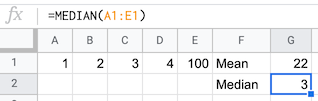
\includegraphics[width=\linewidth, height=0.40\textheight, keepaspectratio]{images/fig_5_1_median_vs_mean.png}\\[0.08cm]
{\fontsize{6.5pt}{7.5pt}\selectfont \textcolor{navyMuted}{\textit{Hình 5.1: Minh họa Mean nhảy vọt lên 22 trong khi Median giữ vững ở 3.}}}
\end{column}
\end{columns}
\slidenumber{20}
\end{frame}


% ==================== SLIDE 22: TƯƠNG QUAN ≠ NHÂN QUẢ ====================
\begin{frame}[plain, t]
\slideheader{Chương 5 • Ngôn Từ Chuẩn Xác}{Tương Quan Không Đồng Nghĩa Với Nhân Quả}
\begin{columns}[T]
\begin{column}{0.54\textwidth}
{\fontsize{8.2pt}{10.5pt}\selectfont
\textbf{Cực kỳ thận trọng với các động từ mang tính áp đặt:}
\textit{``dẫn đến'' (leads to)}, \textit{``thúc đẩy'' (promotes)}, \textit{``gây ra'' (causes)}.

\begin{itemize}\setlength{\itemsep}{2pt}
    \item \textbf{Tương quan (Correlation):} Hai biến số cùng biến thiên trên biểu đồ (ví dụ: tuổi thọ càng cao thì tỷ lệ sinh càng thấp).
    \item \textbf{Nhân quả (Causation):} Biến độc lập trực tiếp tạo ra sự thay đổi ở biến phụ thuộc.
\end{itemize}

\vspace{0.12cm}
\textbf{3 bước bắt buộc để khẳng định Quan hệ Nhân quả:}
\begin{enumerate}\setlength{\itemsep}{1.5pt}
    \item Chứng minh có \textbf{tương quan thống kê rõ rệt}.
    \item Xây dựng \textbf{lý thuyết cơ chế tác động} thuyết phục.
    \item \textbf{Cô lập hoàn toàn mọi biến gây nhiễu (Confounding variables)} -- yếu tố ẩn tác động đồng thời lên cả hai biến.
\end{enumerate}
}
\end{column}
\begin{column}{0.42\textwidth}
\centering
\begin{tikzpicture}[scale=0.9]
    \node[draw=navyMain, fill=boxBg, rounded corners=4pt, align=center, font=\scriptsize\bfseries] (C) at (0, 2.0) {Biến Gây Nhiễu Ẩn\\(Confounding C)};
    \node[draw=navyMain, fill=white, rounded corners=4pt, align=center, font=\scriptsize\bfseries] (A) at (-1.8, 0) {Biến A\\(Quan sát)};
    \node[draw=navyMain, fill=white, rounded corners=4pt, align=center, font=\scriptsize\bfseries] (B) at (1.8, 0) {Biến B\\(Quan sát)};
    \draw[{Latex[length=2mm]}-{Latex[length=2mm]}, dashed, line width=1.1pt, accentRed] (A) -- (B);
    \node[font=\tiny\bfseries, color=accentRed] at (0, -0.55) {Tương quan biểu kiến};
    \draw[-{Latex[length=2.5mm]}, line width=1.2pt, navyMain] (C) -- (A) node[midway, left, font=\tiny] {Tác động};
    \draw[-{Latex[length=2.5mm]}, line width=1.2pt, navyMain] (C) -- (B) node[midway, right, font=\tiny] {Tác động};
\end{tikzpicture}\\[0.15cm]
{\fontsize{6.8pt}{8pt}\selectfont \textcolor{navyMuted}{\textit{Sơ đồ tam giác: A và B tương quan chỉ vì cùng bị C chi phối!}}}
\end{column}
\end{columns}
\slidenumber{22}
\end{frame}
% ==================== SLIDE 24: CHUẨN HÓA KHÁC ====================
\begin{frame}[plain, t]
\slideheader{Chương 5 • Chuẩn Hóa Dữ Liệu}{Các Phương Pháp Chuẩn Hóa \& Ngoại Lệ}
\begin{columns}[T]
\begin{column}{0.51\textwidth}
{\fontsize{8.2pt}{10.5pt}\selectfont
\textbf{Các kỹ thuật chuẩn hóa chuyên sâu khác:}
\begin{itemize}\setlength{\itemsep}{2pt}
    \item \textbf{1. Điều chỉnh theo lạm phát:}
    Không thể so thu nhập \$10.000 năm 1970 với năm 2020. Phải quy đổi từ số danh nghĩa sang sức mua thực tế.
    \item \textbf{2. Điều chỉnh theo mùa vụ:}
    Loại bỏ biến động chu kỳ tự nhiên (du lịch mùa hè, bán lẻ dịp Giáng sinh) để thấy xu hướng thực chất.
    \item \textbf{3. Chỉ số hóa:}
    Đưa các biến có đơn vị khác nhau về cùng mốc chuẩn Base 100 hoặc độ lệch chuẩn.
\end{itemize}
}
\end{column}
\begin{column}{0.45\textwidth}
\calloutbox[\linewidth]{Khi Nào KHÔNG CẦN Chuẩn Hóa?}{
    Khi biến số bản thân nó đã là một \textbf{đại lượng đo lường trên thang quy chiếu chung}:\\[0.1cm]
    • \textbf{Độ tuổi trung vị (Median Age):} Con người ở mọi thành phố đều sống trong thang tuổi 0--120, có thể so sánh trực tiếp.\\
    • \textbf{Thu nhập hộ gia đình trung vị:} Xét trong cùng 1 năm và 1 đơn vị tiền tệ có thể đối chiếu giữa các vùng mà không cần chia theo đầu người!
}
\end{column}
\end{columns}
\slidenumber{24}
\end{frame}

% ==================== SLIDE 25: SELECTION & NON-RESPONSE ====================
\begin{frame}[plain, t]
\slideheader{Chương 5 • Bẫy Chọn Mẫu}{Thiên Vị Chọn Mẫu \& Không Phản Hồi}
\begin{columns}[T]
\begin{column}{0.52\textwidth}
{\fontsize{8pt}{10.2pt}\selectfont
\vspace{0.08cm}
\textbf{1. Thiên vị chọn mẫu }
\begin{itemize}\setlength{\itemsep}{1pt}
    \item Mẫu được chọn khác biệt có hệ thống so với tổng thể.
    \item \textbf{Ví dụ:} Đứng trước cửa phòng Gym để đo chiều cao ngẫu nhiên $\rightarrow$ kết luận sai rằng dân số cao vượt trội!
\end{itemize}

\vspace{0.08cm}
\textbf{2. Thiên vị không phản hồi}
\begin{itemize}\setlength{\itemsep}{1pt}
    \item Người từ chối trả lời khác biệt người trả lời.
    \item \textbf{Thực tế:} Census 2020 trong đại dịch, người nghèo ít phản hồi $\rightarrow$ thu nhập trung vị bị đội lên cao giả tạo.
\end{itemize}
\textbf{3. Thiên vị tự lựa chọn}
\begin{itemize}\setlength{\itemsep}{2pt}
    \item Xảy ra khi đánh giá hiệu quả chương trình nơi người tham gia \textbf{tự nguyện đăng ký} (giảm cân, học bổng).
    \item \textcolor{accentRed}{\textbf{So sánh SAI:}} So sánh người không tham gia (Nhóm A) với người tự đăng ký (Nhóm B).
    \item \textit{Lý do:} Nhóm B vốn đã có \textbf{động lực và ý thức cao hơn hẳn} Nhóm A!
\end{itemize}

}
\end{column}
\begin{column}{0.44\textwidth}
\centering
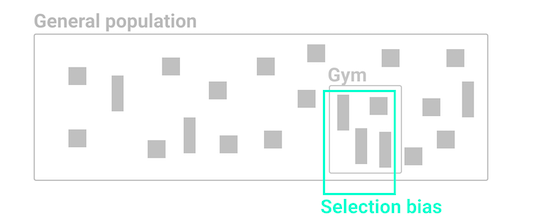
\includegraphics[width=\linewidth, height=0.44\textheight, keepaspectratio]{images/fig_5_2_selection_bias.png}\\[0.08cm]
{\fontsize{6.5pt}{7.5pt}\selectfont \textcolor{navyMuted}{\textit{Hình 5.2: Khung Gym chỉ toàn người cao so với tổng thể chung.}}}
\end{column}
\end{columns}
\slidenumber{25}
\end{frame}

% ==================== BẮT ĐẦU PHẦN 2 ====================
% ==================== SLIDE 1 ====================
\begin{frame}[plain,c]
\begin{tikzpicture}[remember picture,overlay]
\node[anchor=north west] at ($(current page.north west)+(1.0cm,-0.8cm)$) {\textcolor{navyMuted}{\fontsize{8.5pt}{10.5pt}\selectfont Tháng 10, 2026}};
\node[anchor=west,text width=0.96\textwidth] at ($(current page.west)+(1.0cm,0.3cm)$) {
{\fontsize{13pt}{15pt}\selectfont\bfseries\color{navyMuted}PHẦN 2 • BÁO CÁO CHUYÊN ĐỀ}\\[0.25cm]
{\fontsize{28pt}{32pt}\selectfont\bfseries\color{navyMain}TRỰC QUAN HÓA}\\[0.12cm]
{\fontsize{28pt}{32pt}\selectfont\bfseries\color{navyMain}BIỂU ĐỒ}\\[0.18cm]
{\fontsize{20pt}{24pt}\selectfont\bfseries\color{navyMain}CHART YOUR DATA}\\[0.35cm]
{\fontsize{10pt}{13pt}\selectfont Chương 6\\[0.15cm]Chọn đúng dạng • Đọc đúng thang • Làm rõ dữ liệu}
};
\end{tikzpicture}
\note{Chương 6 tập trung vào chọn loại biểu đồ theo dữ liệu và câu chuyện, đọc đúng thang đo và thiết kế rõ ràng. Nguồn: sách trang 121--126; \url{https://handsondataviz.org/chart.html}.}
\slidenumber{01}\end{frame}
% ==================== SLIDE 2 ====================
\begin{frame}[plain,t]
\slideheader{Chương 6 • Chart Your Data}{Chọn Biểu Đồ Từ Câu Hỏi}
{\bodytext Loại biểu đồ phụ thuộc \textbf{dữ liệu và câu chuyện}.\par}\vspace{0.18cm}\vspace{0.25cm}
\begin{columns}[T,onlytextwidth]
\begin{column}{.47\textwidth}
\briefdef{So sánh}{→ Thanh / cột}
\briefdef{Phân bố}{→ Histogram}
\briefdef{Thời gian}{→ Đường}
\end{column}
\begin{column}{.47\textwidth}
\briefdef{Chênh lệch}{→ Range}
\briefdef{Quan hệ}{→ Phân tán}
\end{column}
\end{columns}
\vspace{0.40cm}\takeaway{Đôi khi bảng hoặc một câu văn đã đủ.}
\note{Đặt câu hỏi trước khi chọn loại biểu đồ. Dữ liệu danh mục, chuỗi thời gian hay nhiều biến cần cách biểu diễn khác nhau. Nguyên tắc thiết kế cần được đánh giá theo sự trung thực và khả năng đọc, không áp dụng máy móc cho mọi trường hợp. Bảng tra cứu chi tiết trong sách trang 122--125. Nguồn: \url{https://handsondataviz.org/chart.html}; \url{https://handsondataviz.org/chart-design.html}.}
\slidenumber{02}
\end{frame}

% ==================== SLIDE 3 ====================
\begin{frame}[plain,t]
\slideheader{Chương 6 • Chart Your Data}{Biểu Đồ Cần Gì Để Đọc Đúng?}
\begin{columns}[T,onlytextwidth]
\begin{column}{.30\textwidth}
\briefdef{Tiêu đề:}{thông điệp}
\briefdef{Trục:}{thang đo và đơn vị}
\briefdef{Nhãn / chú giải:}{cách đọc giá trị}
\briefdef{Nguồn / ghi chú:}{bối cảnh}
\end{column}
\begin{column}{.66\textwidth}
\centering 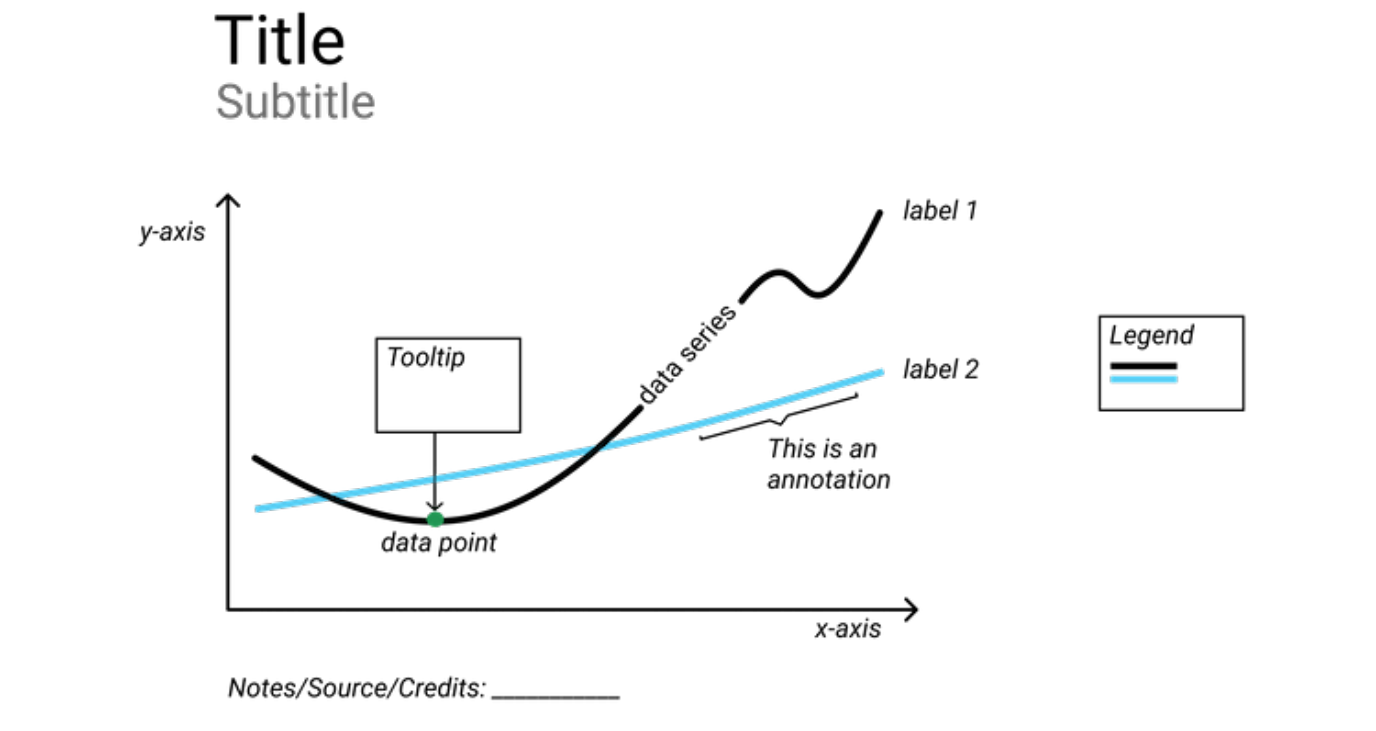
\includegraphics[width=\linewidth,height=.51\textheight,keepaspectratio]{images/part2_book/fig_6_1.png}\\[0.08cm]\figcaption{Các thành phần của biểu đồ}
\end{column}\end{columns}\takeaway{Thông tin cốt lõi phải hiện ra, không chỉ nằm trong hộp thông tin (tooltip).}
\note{Tiêu đề có thể nêu thông điệp, kết hợp phụ đề kỹ thuật ngắn mô tả biến, địa điểm và thời gian. Nếu bất định đã biết, thể hiện bằng thanh sai số khi phù hợp hoặc ghi hạn chế; không phải mọi dữ liệu mẫu đều bắt buộc vẽ chữ I. Tooltip chỉ bổ sung vì có thể mất khi in và khó tương tác trên điện thoại. Hình 6.1, sách trang 127; nội dung trang 126--128. \url{https://handsondataviz.org/chart-design.html}.}
\slidenumber{03}
\end{frame}

% ==================== SLIDE 4 ====================
\begin{frame}[plain,t]
\slideheader{Chương 6 • Chart Your Data}{Gốc 0 Phụ Thuộc Cách Mã Hóa}
\begin{columns}[T,onlytextwidth]
\begin{column}{.48\textwidth}
{\bodytext \textbf{Thanh / cột / miền}\\Chiều dài hoặc diện tích → bắt đầu từ 0.\par}\vspace{0.18cm}\centering 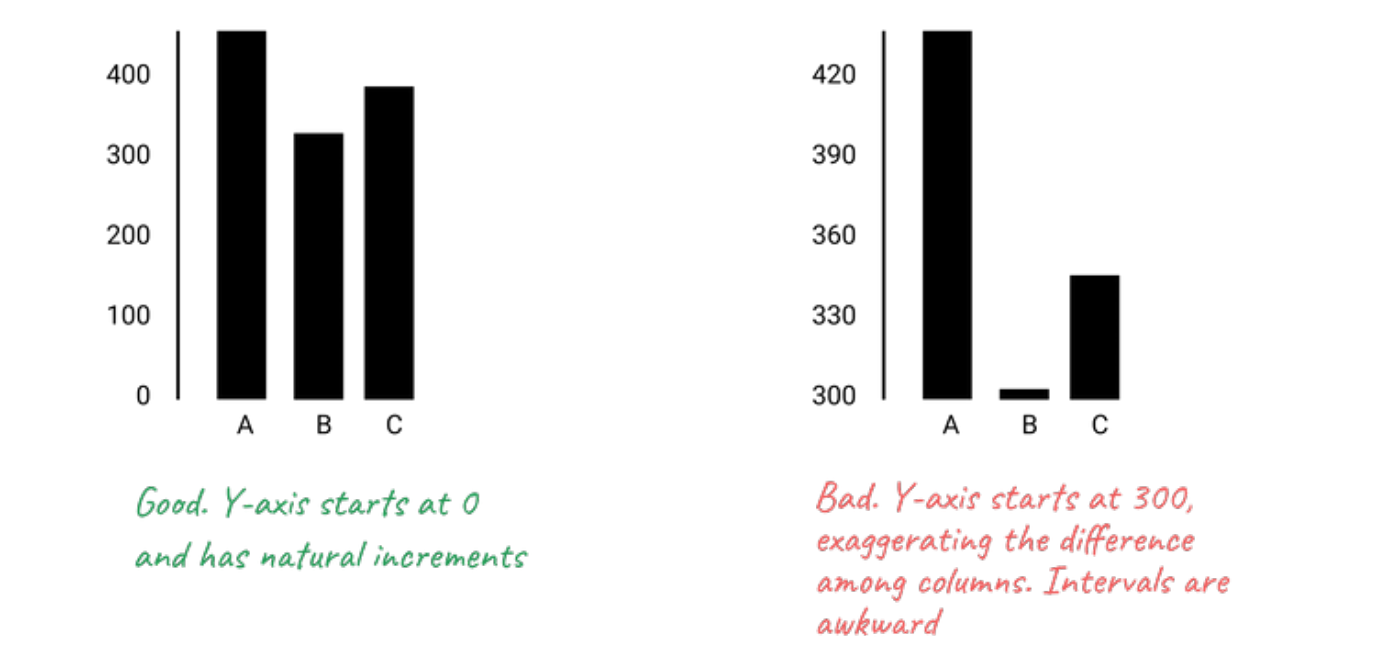
\includegraphics[width=\linewidth,height=.32\textheight,keepaspectratio]{images/part2_book/fig_6_2.png}\\[0.08cm]\figcaption{Cột: gốc 0 và trục bị cắt}
\end{column}
\begin{column}{.48\textwidth}
{\bodytext \textbf{Đường}\\Vị trí của điểm → không bắt buộc gốc 0.\par}\vspace{0.18cm}\centering 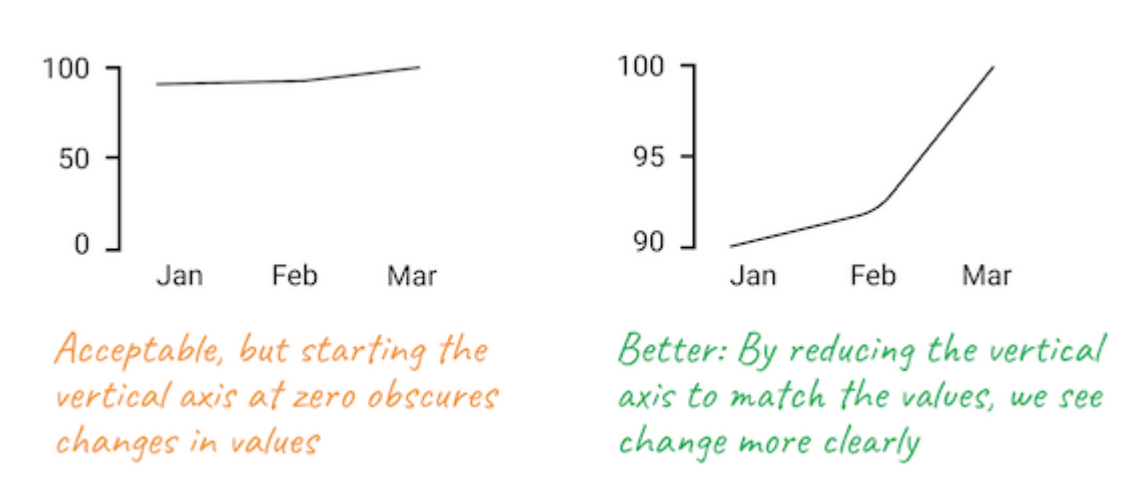
\includegraphics[width=\linewidth,height=.32\textheight,keepaspectratio]{images/part2_book/fig_6_4.png}\\[0.08cm]\figcaption{Đường: điều chỉnh khoảng trục}
\end{column}\end{columns}\takeaway{Với biểu đồ đường, chọn giới hạn trục phù hợp và ghi rõ thang đo.}
\note{Cột dùng chiều dài nên phải giữ gốc 0, tương tự vùng tô diện tích. Đường mã hóa vị trí điểm nên có thể điều chỉnh khoảng trục để đọc biến động. Trục đường từ 0 vẫn có thể chấp nhận; cả hai cách đều có thể trung thực. Không quy kết ý định lừa dối chỉ vì trục đường không bắt đầu từ 0. Hình 6.2 trang 128 và hình 6.4 trang 130. \url{https://handsondataviz.org/chart-design.html}.}
\slidenumber{04}
\end{frame}

% ==================== SLIDE 5 ====================
\begin{frame}[plain,t]
\slideheader{Chương 6 • Chart Your Data}{Biểu Đồ Tròn Thể Hiện Một Tổng 100\%}
{\bodytext Mỗi lát là một phần của \textbf{cùng tổng thể}.\par}\vspace{0.18cm}\begin{columns}[T,onlytextwidth]
\begin{column}{.48\textwidth}
\centering 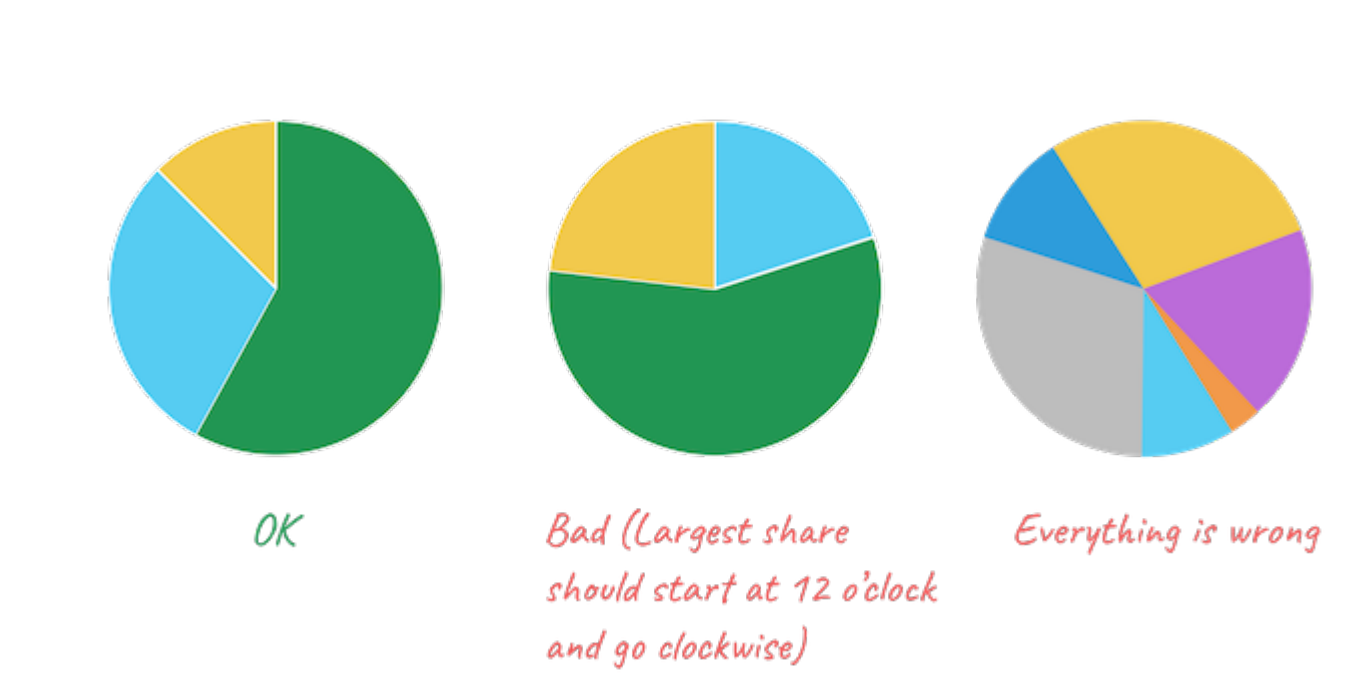
\includegraphics[width=\linewidth,height=.34\textheight,keepaspectratio]{images/part2_book/fig_6_6.png}\\[0.08cm]\figcaption{Các phần phải cộng thành 100\%}
\end{column}
\begin{column}{.48\textwidth}
\centering 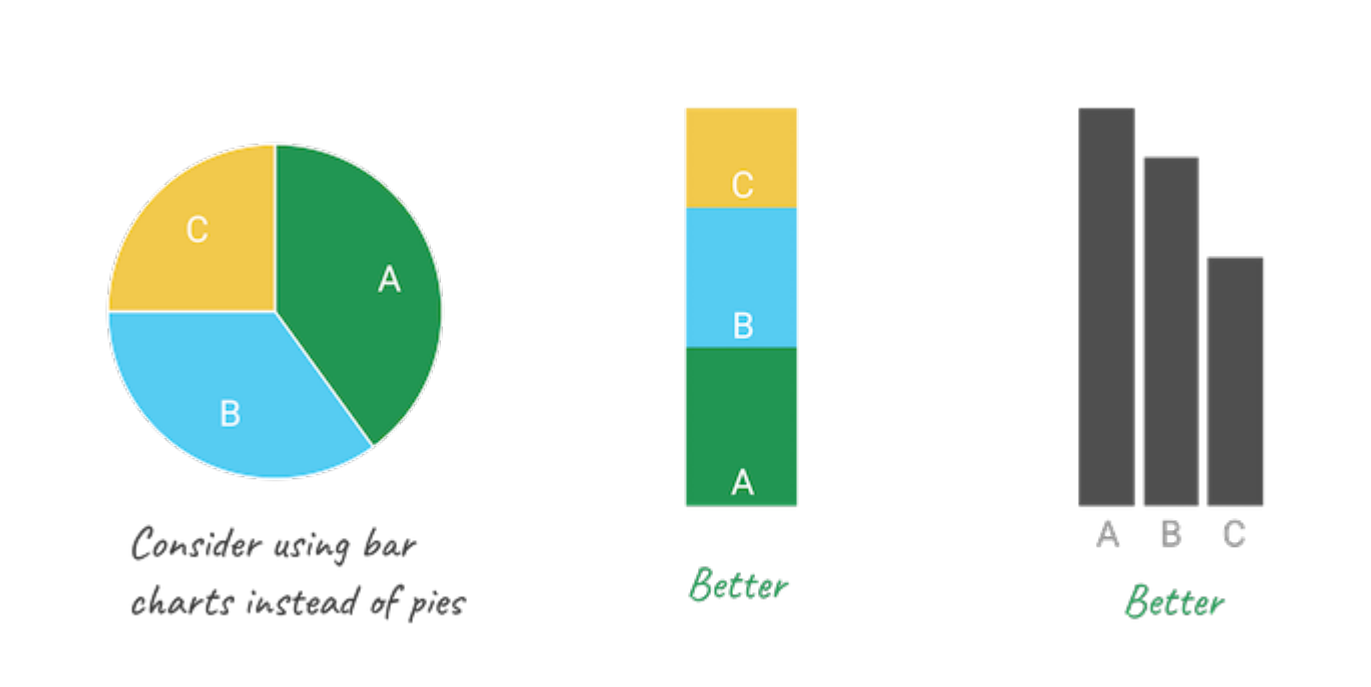
\includegraphics[width=\linewidth,height=.34\textheight,keepaspectratio]{images/part2_book/fig_6_7.png}\\[0.08cm]\figcaption{Khó so sánh? Cân nhắc thanh}
\end{column}\end{columns}\takeaway{100\%: điều kiện cần • Ít lát: dễ đọc hơn}
\note{Biểu đồ tròn cần các phần của cùng tổng thể và tổng bằng 100 phần trăm. Khảo sát cho phép chọn nhiều đáp án thường không đáp ứng điều kiện này. Sách khuyên không quá năm lát và sắp từ 12 giờ theo chiều kim đồng hồ; đây là khuyến nghị về khả năng đọc. Thanh giúp so sánh các phần có giá trị gần nhau. Hình 6.6 trang 131 và hình 6.7 trang 132. \url{https://handsondataviz.org/chart-design.html}.}
\slidenumber{05}
\end{frame}

% ==================== SLIDE 6 ====================
\begin{frame}[plain,t]
\slideheader{Chương 6 • Chart Your Data}{Giữ Điều Giúp Người Xem Đọc Rõ}
{\bodytext \textbf{Rác đồ họa:} yếu tố trang trí làm giảm khả năng đọc.\par}\vspace{0.18cm}\begin{columns}[T,onlytextwidth]
\begin{column}{.30\textwidth}
\briefdef{Bỏ}{3D / bóng đổ thừa}
\briefdef{Nhãn dài}{→ Thanh ngang}
\briefdef{Sắp xếp}{có lý do}
\briefdef{Màu}{có mục đích}
\end{column}
\begin{column}{.66\textwidth}
\centering 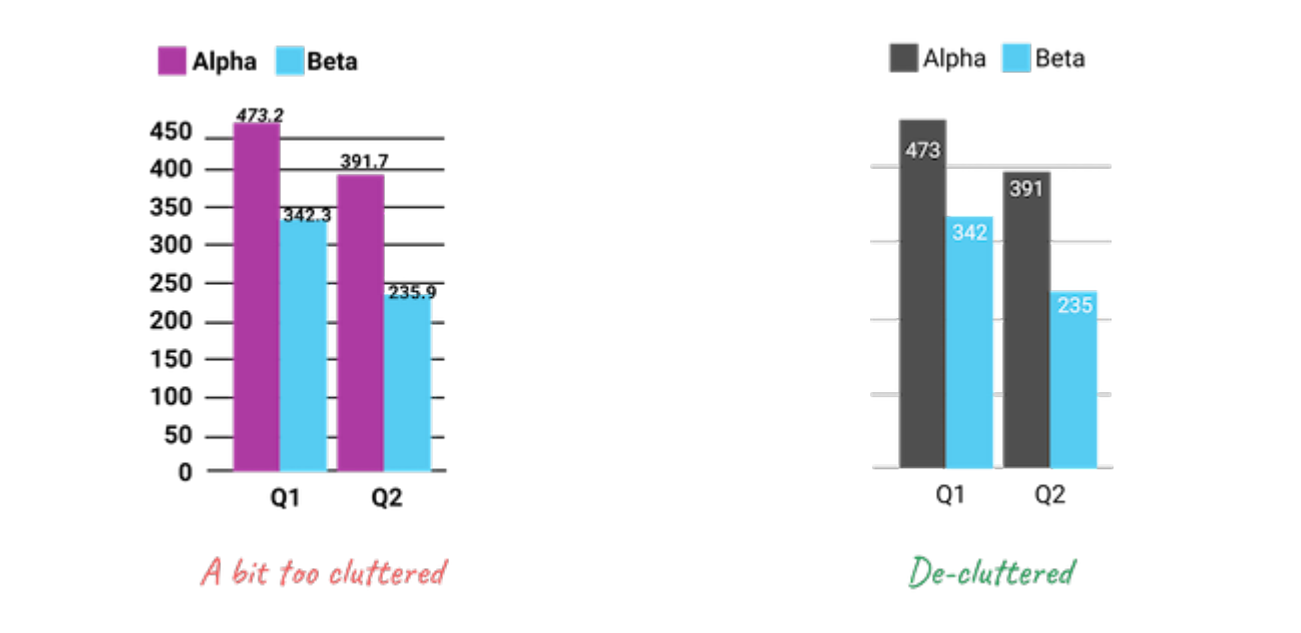
\includegraphics[width=\linewidth,height=.51\textheight,keepaspectratio]{images/part2_book/fig_6_11.png}\\[0.08cm]\figcaption{Tinh giản để làm rõ dữ liệu}
\end{column}\end{columns}\takeaway{Kiểm tra khả năng phân biệt màu và bản in trắng đen.}
\note{Giảm trang trí không phục vụ đọc dữ liệu. Tránh 3D giả tạo làm méo cảm nhận; điều này không cấm biểu diễn dữ liệu thực sự ba chiều. Nhãn dài phù hợp thanh ngang. Sắp xếp theo giá trị hay thứ tự có lý do. Màu có ý nghĩa theo ngữ cảnh và văn hóa; không mặc định đỏ luôn xấu và xanh luôn tốt. Kiểm tra người có khác biệt thị giác màu và bản in thang xám. Hình 6.11 trang 135. \url{https://handsondataviz.org/chart-design.html}.}
\slidenumber{06}
\end{frame}

% ==================== SLIDE 7 ====================
\begin{frame}[plain,t]
\slideheader{Chương 6 • Chart Your Data}{Ba Cách So Sánh Danh Mục}
\begin{columns}[T,onlytextwidth]
\begin{column}{.315\textwidth}\briefdef{Nhóm}{Đặt cạnh nhau}
\centering 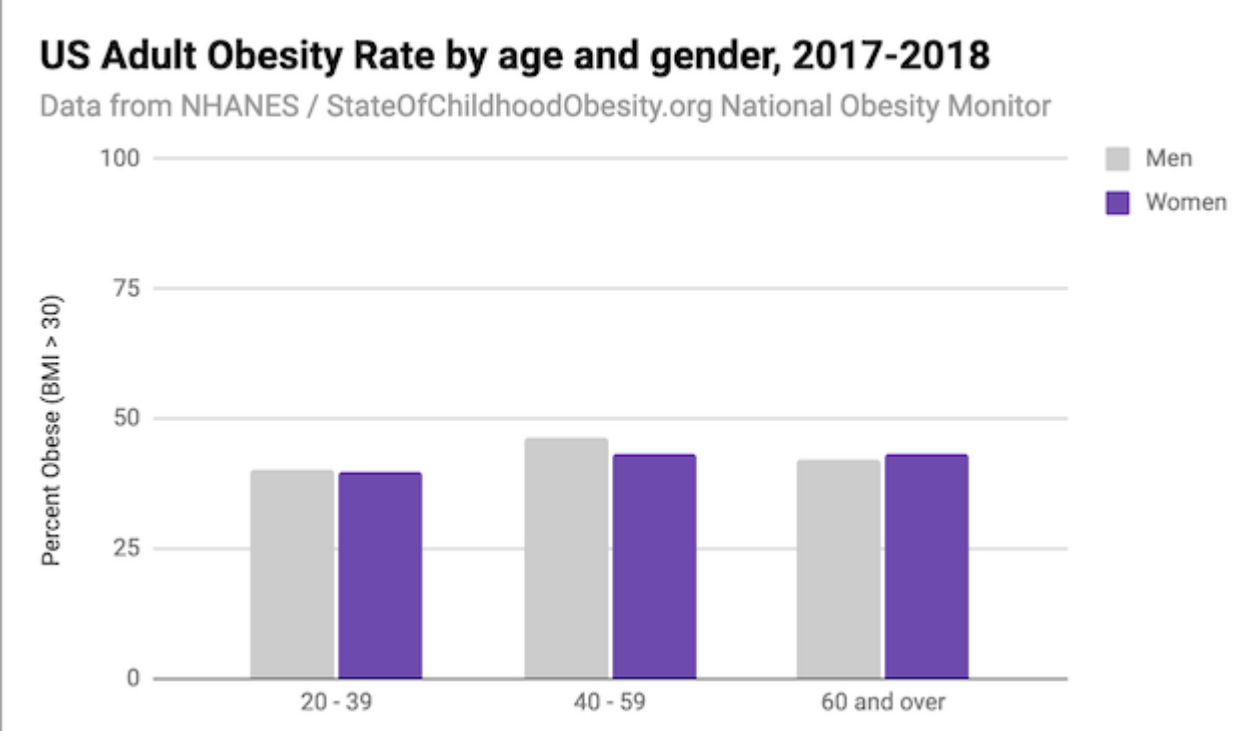
\includegraphics[width=\linewidth,height=.32\textheight,keepaspectratio]{images/part2_book/fig_6_13.png}\\[0.08cm]\figcaption{Béo phì theo tuổi / giới}\end{column}
\begin{column}{.315\textwidth}\briefdef{Tách}{Chia thành cụm}
\centering 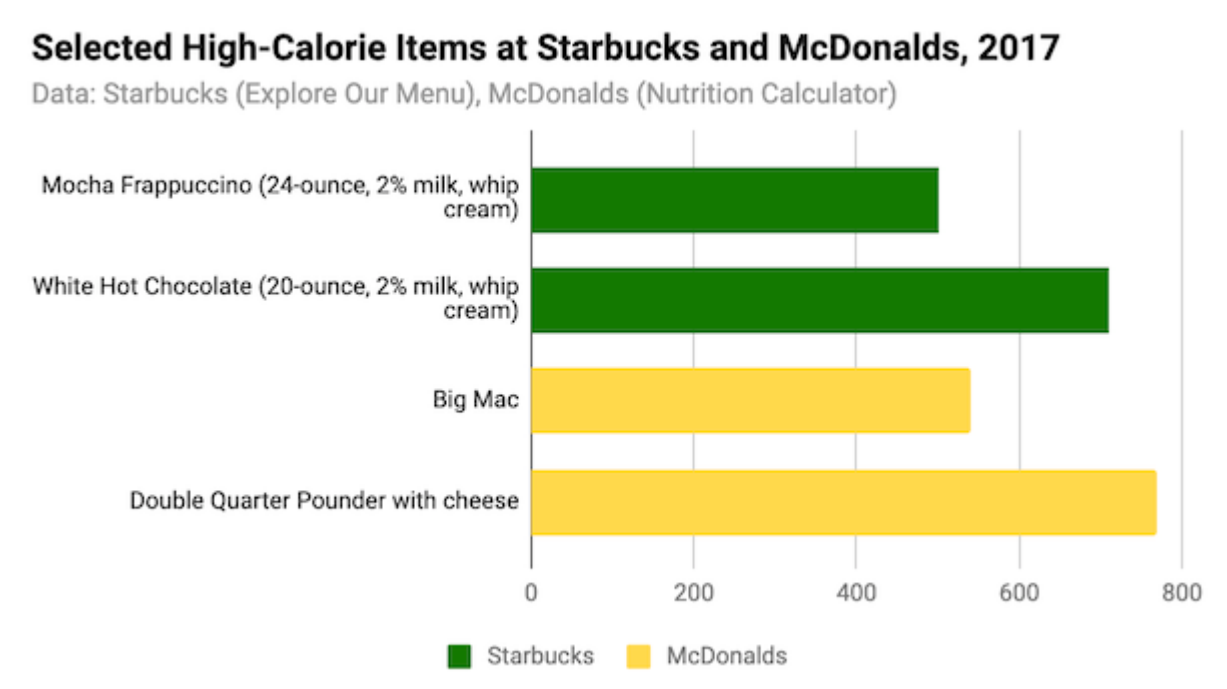
\includegraphics[width=\linewidth,height=.32\textheight,keepaspectratio]{images/part2_book/fig_6_23.png}\\[0.08cm]\figcaption{Calo món ăn theo nhà hàng}\end{column}
\begin{column}{.315\textwidth}\briefdef{Chồng}{Thành phần trong tổng}
\centering 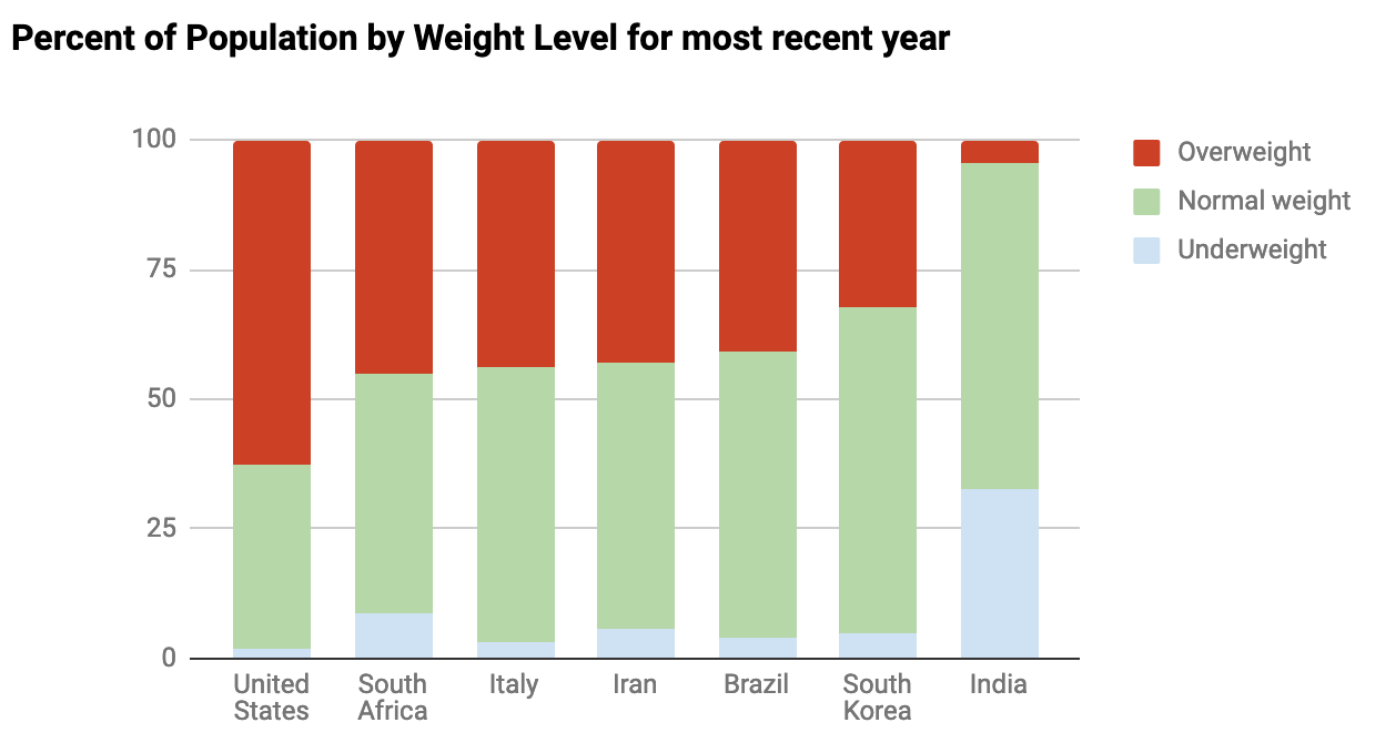
\includegraphics[width=\linewidth,height=.32\textheight,keepaspectratio]{images/part2_book/fig_6_25.png}\\[0.08cm]\figcaption{Nhóm cân nặng theo quốc gia}\end{column}
\end{columns}\takeaway{Cách bố trí phụ thuộc điều cần so sánh.}
\note{Nhóm đặt các cột cạnh nhau. Tách trong ví dụ sách là các cụm riêng vì danh sách món ăn của hai nhà hàng khác nhau; không đồng nhất với các đồ thị con độc lập cùng trục. Chồng thể hiện các thành phần trong tổng; phần ở đáy có cùng gốc nên dễ so sánh hơn các phần phía trên. Hình 6.13 trang 137 dùng NHANES 2017--2018; hình 6.23 trang 142 dùng thực đơn Starbucks và McDonalds; hình 6.25 trang 144 dùng WHO và CDC. Nguồn: Chương 6, sách trang 136--144.}
\slidenumber{07}
\end{frame}

% ==================== SLIDE 8 ====================
\begin{frame}[plain,t]
\slideheader{Chương 6 • Chart Your Data}{Histogram Cho Thấy Phân Bố}
{\bodytext Đếm số giá trị rơi vào từng \textbf{khoảng (bin)}.\par}\vspace{0.18cm}\begin{columns}[T,onlytextwidth]
\begin{column}{.30\textwidth}
{\bodytext\textbf{Trung tâm}\\[0.25cm]\textbf{Độ phân tán}\\[0.25cm]\textbf{Giá trị ở hai đuôi}\par}
\end{column}
\begin{column}{.66\textwidth}
\centering 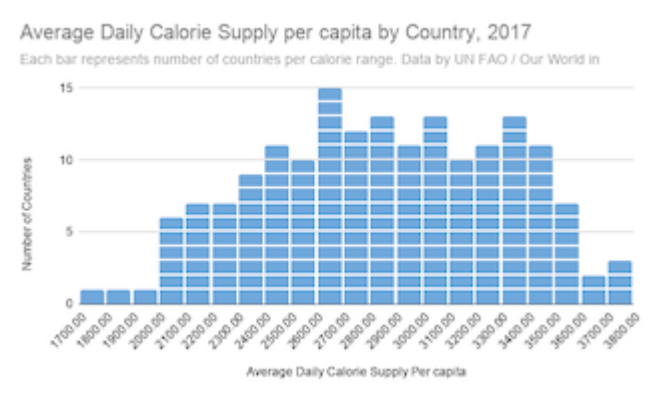
\includegraphics[width=\linewidth,height=.51\textheight,keepaspectratio]{images/part2_book/fig_6_28.png}\\[0.08cm]\figcaption{Nguồn cung calo/người/ngày • 174 quốc gia • 2017}
\end{column}\end{columns}\takeaway{Nguồn cung thực phẩm không đồng nghĩa lượng thực sự ăn.}
\note{Histogram đếm quan sát theo khoảng giá trị, thay vì mỗi cột là một danh mục. Ví dụ FAO qua Our World in Data năm 2017 gồm 174 quốc gia, đo nguồn cung calo bình quân mỗi người mỗi ngày, không đo lượng ăn thực tế. Đỉnh khoảng 2800 kcal; tám nước dưới 2000 và mười một nước trên 3500. Không từ đó gán nhãn đói nghèo hay dư thừa. Kích thước bin ảnh hưởng hình dạng quan sát, nên thử cách chia hợp lý. Hình 6.28 trang 146. \url{https://handsondataviz.org/histogram-google.html}.}
\slidenumber{08}
\end{frame}

% ==================== SLIDE 9 ====================
\begin{frame}[plain,t]
\slideheader{Chương 6 • Chart Your Data}{Đường Xem Từng Chuỗi, Miền Chồng Xem Tổng}
\begin{columns}[T,onlytextwidth]
\begin{column}{.48\textwidth}
{\bodytext \textbf{Đường:} giá trị thay đổi\\theo thời gian.\par}\vspace{0.18cm}\centering 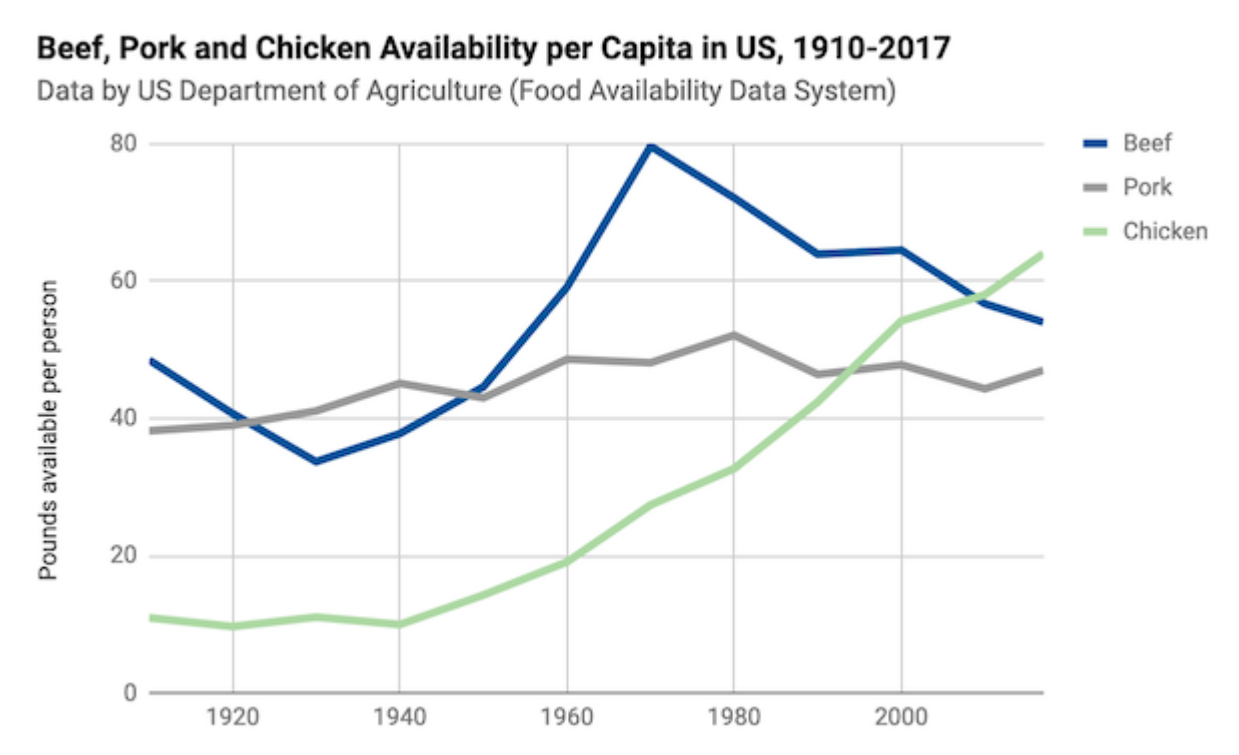
\includegraphics[width=\linewidth,height=.35\textheight,keepaspectratio]{images/part2_book/fig_6_33.png}\\[0.08cm]\figcaption{Đường → So từng loại}
\end{column}
\begin{column}{.48\textwidth}
{\bodytext \textbf{Miền chồng:} thành phần và tổng thay đổi theo thời gian.\par}\vspace{0.18cm}\centering 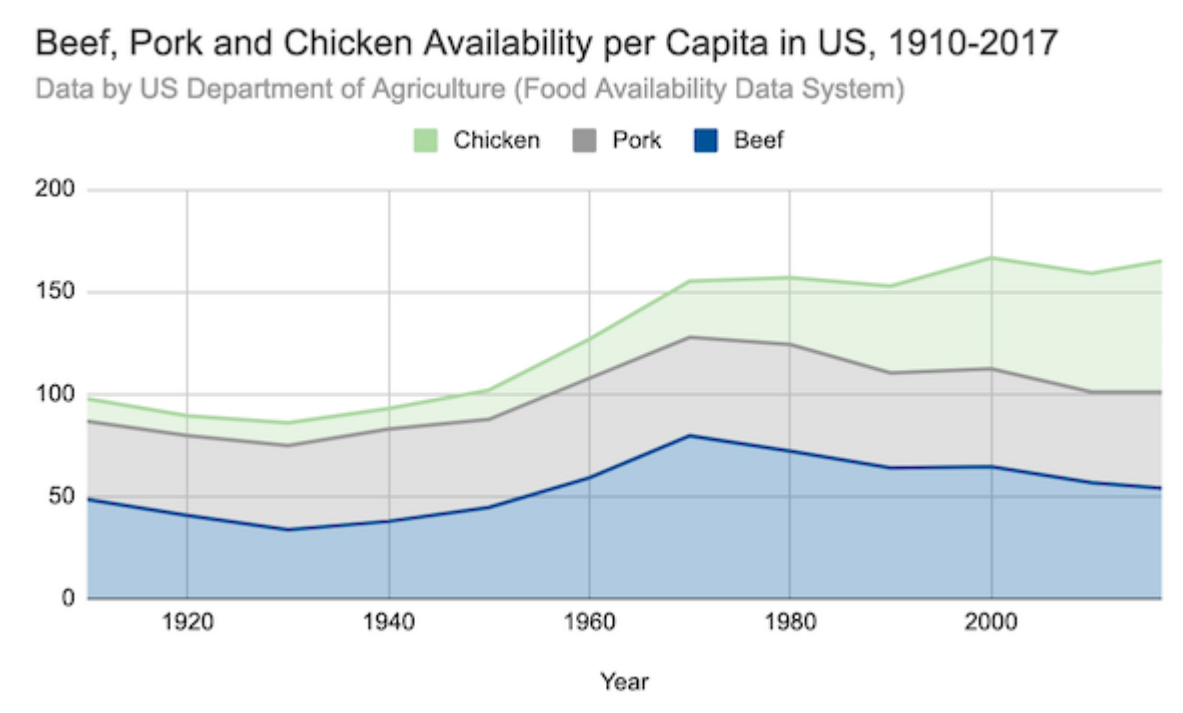
\includegraphics[width=\linewidth,height=.35\textheight,keepaspectratio]{images/part2_book/fig_6_34.png}\\[0.08cm]\figcaption{Miền chồng → Thấy tổng}
\end{column}\end{columns}\takeaway{Lượng thịt sẵn có bình quân đầu người tại Mỹ • USDA}
\note{Dữ liệu USDA đo lượng thực phẩm sẵn có bình quân đầu người, không phải lượng tiêu thụ thực tế. Đường giúp đọc từng loại và các giao cắt; thịt gà vượt thịt bò và thịt lợn quanh năm 2000, không nên khẳng định chính xác năm nếu hình không chứng minh. Miền chồng làm rõ cả tổng và thành phần; đường không làm tổng bất khả thi nhưng khó thấy trực tiếp. Có thể thêm chú thích sự kiện và bộ lọc để giảm quá tải, như các ví dụ thất nghiệp và sử dụng Internet trong sách. Hình 6.33 trang 151 và 6.34 trang 152. \url{https://handsondataviz.org/pie-line-area-google.html}.}
\slidenumber{09}
\end{frame}

% ==================== SLIDE 10 ====================
\begin{frame}[plain,t]
\slideheader{Chương 6 • Chart Your Data}{Range Làm Rõ Chênh Lệch}
{\bodytext Hai điểm và đoạn nối nhấn \textbf{chênh lệch giữa các nhóm}.\par}\vspace{0.18cm}\centering 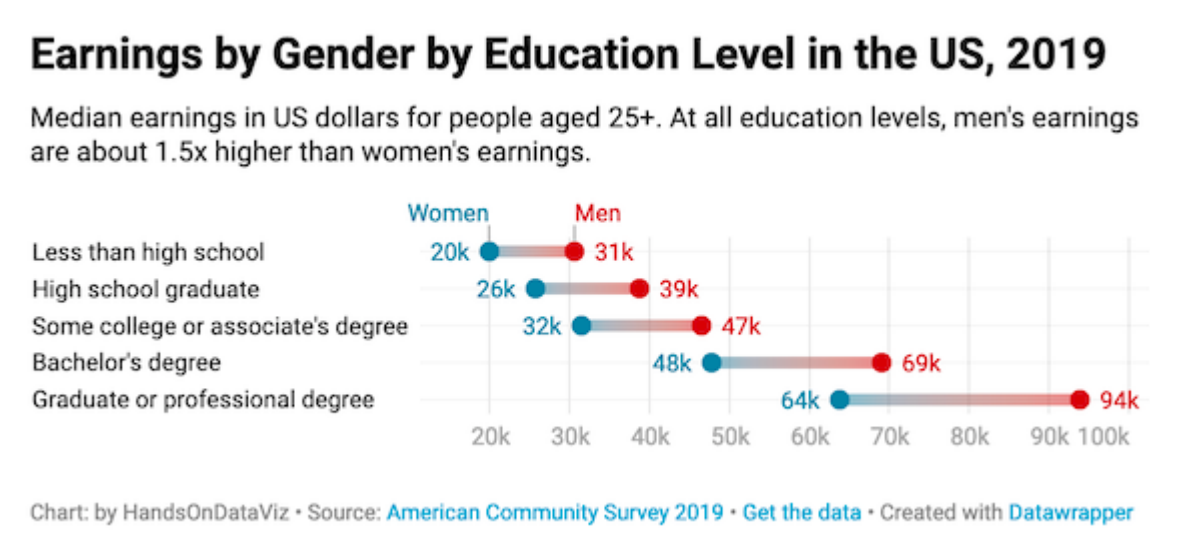
\includegraphics[width=.95\linewidth,height=.54\textheight,keepaspectratio]{images/part2_book/fig_6_39.png}\\[0.08cm]\figcaption{Thu nhập trung vị theo giới và học vấn • Mỹ, ACS 2019}\takeaway{Chênh lệch vẫn hiện ở từng bậc học.}
\note{Ví dụ là thu nhập trung vị của người từ 25 tuổi trở lên, theo giới và trình độ học vấn trong ACS 2019. Nam có bằng cử nhân khoảng 69 nghìn USD, nữ có bằng sau đại học hoặc chuyên môn khoảng 64 nghìn USD. Không diễn giải thành mọi cá nhân hay chênh lệch lương đã điều chỉnh yếu tố khác; cũng không suy luận nhân quả. Thu nhập trung vị theo nhóm không mô tả mọi cá nhân. Hình 6.39 trang 158. \url{https://handsondataviz.org/range-datawrapper.html}.}
\slidenumber{10}
\end{frame}

% ==================== SLIDE 11 ====================
\begin{frame}[plain,t]
\slideheader{Chương 6 • Chart Your Data}{Phân Tán Cho Thấy Quan Hệ X–Y}
{\bodytext Mỗi điểm đặt hai giá trị của \textbf{cùng một đối tượng} lên hai trục.\par}\vspace{0.18cm}\begin{columns}[T,onlytextwidth]
\begin{column}{.30\textwidth}
\briefdef{X:}{tuổi thọ}
\briefdef{Y:}{số con / phụ nữ}
\vspace{0.3cm}{\bodytext Tương quan \textbf{không chứng minh nhân quả}.\par}
\end{column}
\begin{column}{.66\textwidth}
\centering 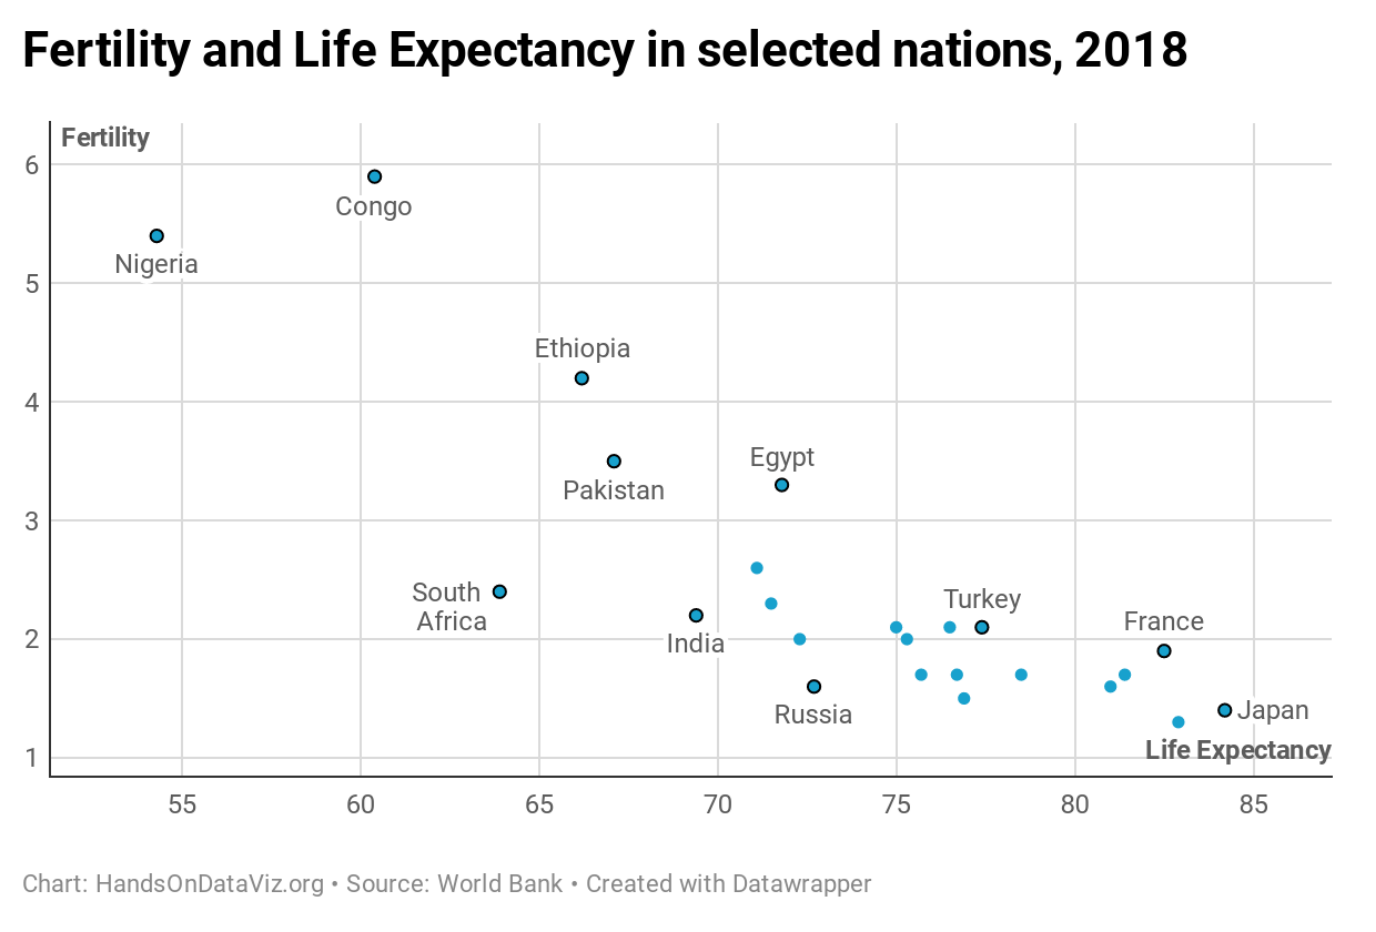
\includegraphics[width=\linewidth,height=.51\textheight,keepaspectratio]{images/part2_book/fig_6_44.png}\\[0.08cm]\figcaption{World Bank 2018 • Mỗi điểm là một quốc gia trong ví dụ}
\end{column}\end{columns}
\note{Biểu đồ thể hiện một số quốc gia được chọn trong dữ liệu World Bank 2018, không phải tất cả quốc gia. Trục X là tuổi thọ, trục Y là số con trên một phụ nữ, không phải số ca sinh trên nghìn dân. Mẫu hình tương quan nghịch không cho phép kết luận sinh ít con làm tăng tuổi thọ. Ví dụ tương quan thuận thu nhập và điểm thi ở Connecticut có thể dùng trong lời nói để đối chiếu, không cần thêm một hình nhỏ trên slide. Hình 6.44 trang 162. \url{https://handsondataviz.org/scatter-bubble-datawrapper.html}.}
\slidenumber{11}
\end{frame}

% ==================== SLIDE 12 ====================
\begin{frame}[plain,t]
\slideheader{Chương 6 • Chart Your Data}{Bong Bóng Thêm Kích Thước Và Màu}
{\bodytext Mở rộng biểu đồ phân tán bằng \textbf{hai biến nữa}.\par}\vspace{0.18cm}\begin{columns}[T,onlytextwidth]
\begin{column}{.30\textwidth}
\briefdef{X:}{tuổi thọ}
\briefdef{Y:}{số con / phụ nữ}
\briefdef{Kích thước:}{dân số}
\briefdef{Màu:}{khu vực}
\end{column}
\begin{column}{.66\textwidth}
\centering 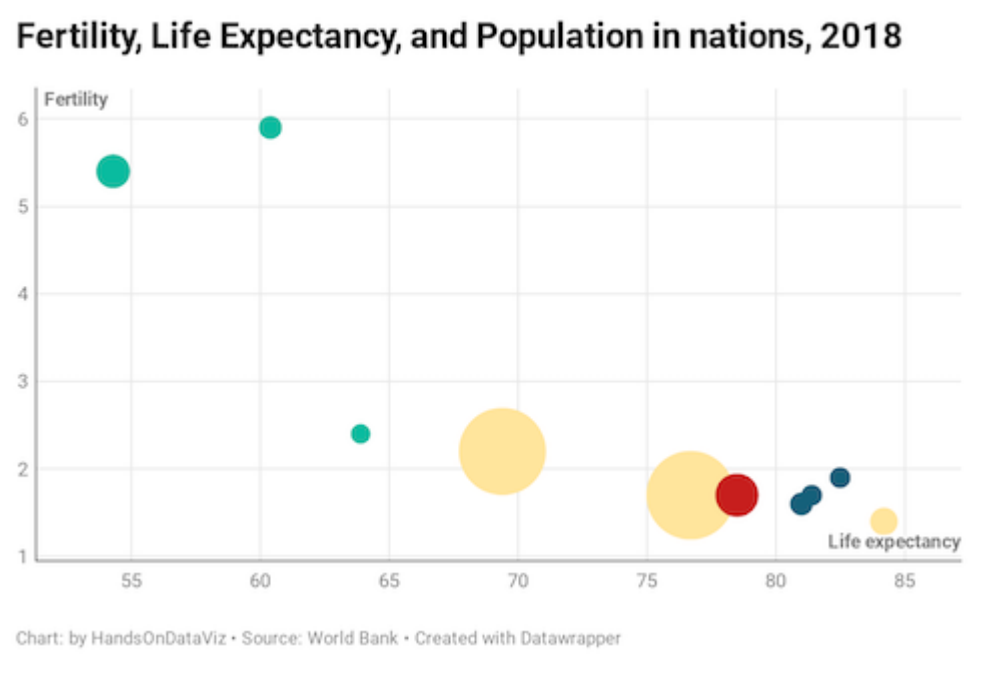
\includegraphics[width=\linewidth,height=.51\textheight,keepaspectratio]{images/part2_book/fig_6_48.png}\\[0.08cm]\figcaption{Tuổi thọ, số con/phụ nữ và dân số • World Bank 2018}
\end{column}\end{columns}\takeaway{Chọn đúng dạng • Giữ đúng thang • Làm rõ điều quan trọng}
\note{Hình dùng các quốc gia được chọn trong World Bank 2018. Bốn biến được mã hóa qua X, Y, kích thước và màu. Tên quốc gia là định danh, không tự động tính thành biến thứ năm. Chuyển động có thể bổ sung thời gian trong một ứng dụng khác nhưng nằm ngoài ví dụ tĩnh này. Kích thước vòng tròn cần đọc theo diện tích, không diễn giải theo bán kính. Kết nối sang phần bản đồ: cùng câu hỏi chọn hình thức biểu diễn phù hợp với dữ liệu. Hình 6.48 trang 165. \url{https://handsondataviz.org/scatter-bubble-datawrapper.html}.}
\slidenumber{12}
\end{frame}

% ==================== BẮT ĐẦU PHẦN 3 ====================
% ==================== SLIDE 1 ====================
\begin{frame}[plain,c]
\begin{tikzpicture}[remember picture,overlay]
\node[anchor=north west] at ($(current page.north west)+(1.0cm,-0.8cm)$) {\textcolor{navyMuted}{\fontsize{8.5pt}{10.5pt}\selectfont Tháng 10, 2026}};
\node[anchor=west,text width=0.96\textwidth] at ($(current page.west)+(1.0cm,0.3cm)$) {
{\fontsize{13pt}{15pt}\selectfont\bfseries\color{navyMuted}PHẦN 3 • BÁO CÁO CHUYÊN ĐỀ}\\[0.25cm]
{\fontsize{28pt}{32pt}\selectfont\bfseries\color{navyMain}TRỰC QUAN HÓA}\\[0.12cm]
{\fontsize{28pt}{32pt}\selectfont\bfseries\color{navyMain}KHÔNG GIAN}\\[0.18cm]
{\fontsize{20pt}{24pt}\selectfont\bfseries\color{navyMain}MAP YOUR DATA}\\[0.35cm]
{\fontsize{10pt}{13pt}\selectfont Chương 7\\[0.15cm]Chọn kiểu bản đồ • Thiết kế màu • So sánh đúng}
};
\end{tikzpicture}
\note{Giới thiệu Chương 7: chọn kiểu bản đồ, thiết kế bản đồ và so sánh dữ liệu có ý nghĩa. Không phải hướng dẫn thao tác từng công cụ. Nguồn: \url{https://handsondataviz.org/map.html}.}
\slidenumber{01}
\end{frame}

% ==================== SLIDE 2 ====================
\begin{frame}[plain,t]
\slideheader{Chương 7 • Map Your Data}{Khi Nào Cần Bản Đồ?}
{\bodytext Vẽ bản đồ khi \textbf{vị trí} giúp làm rõ câu chuyện.\par}
\vspace{0.45cm}
\begin{columns}[T,onlytextwidth]
\begin{column}{0.49\textwidth}
{\fontsize{15pt}{21pt}\selectfont\bfseries Khoảng cách\\[0.32cm]Cụm điểm\\[0.32cm]Phân bố theo vùng\par}
\end{column}
\begin{column}{0.46\textwidth}
\briefdef{So sánh giá trị}{→ Biểu đồ thanh}
\briefdef{Theo thời gian}{→ Biểu đồ đường}
\briefdef{Quan hệ hai biến}{→ Biểu đồ phân tán}
\end{column}
\end{columns}
\vspace{0.40cm}
\takeaway{Có địa chỉ không có nghĩa phải vẽ bản đồ.}
\note{Bản đồ hữu ích khi vị trí và mẫu hình không gian là một phần của câu hỏi. Khoảng cách giữa các điểm, cụm điểm và phân bố theo vùng thường dễ nhận ra trên bản đồ. Nhưng nếu câu hỏi là nơi nào cao nhất thì biểu đồ thanh có thể giúp so sánh chính xác hơn. Dùng biểu đồ đường cho thay đổi theo thời gian, biểu đồ phân tán cho quan hệ hai biến. Không nên hiểu rằng bản đồ không bao giờ thể hiện được hai biến: đây là quyết định dựa trên câu chuyện và mức độ phức tạp. Nguồn: \url{https://handsondataviz.org/map-design.html}.}
\slidenumber{02}
\end{frame}

% ==================== SLIDE 3 ====================
\begin{frame}[plain,t]
\slideheader{Chương 7 • Map Your Data}{Bản Đồ Gồm Nền Và Lớp Dữ Liệu}
\begin{columns}[c,onlytextwidth]
\begin{column}{0.30\textwidth}
\briefdef{Lớp nền:}{bối cảnh địa lý.}
\briefdef{Lớp dữ liệu:}{đối tượng cần thể hiện.}
\vspace{0.15cm}
\briefdef{Điểm:}{một vị trí}
\briefdef{Tuyến:}{chuỗi điểm nối nhau}
\briefdef{Vùng:}{hình khép kín}
\end{column}
\begin{column}{0.66\textwidth}\centering
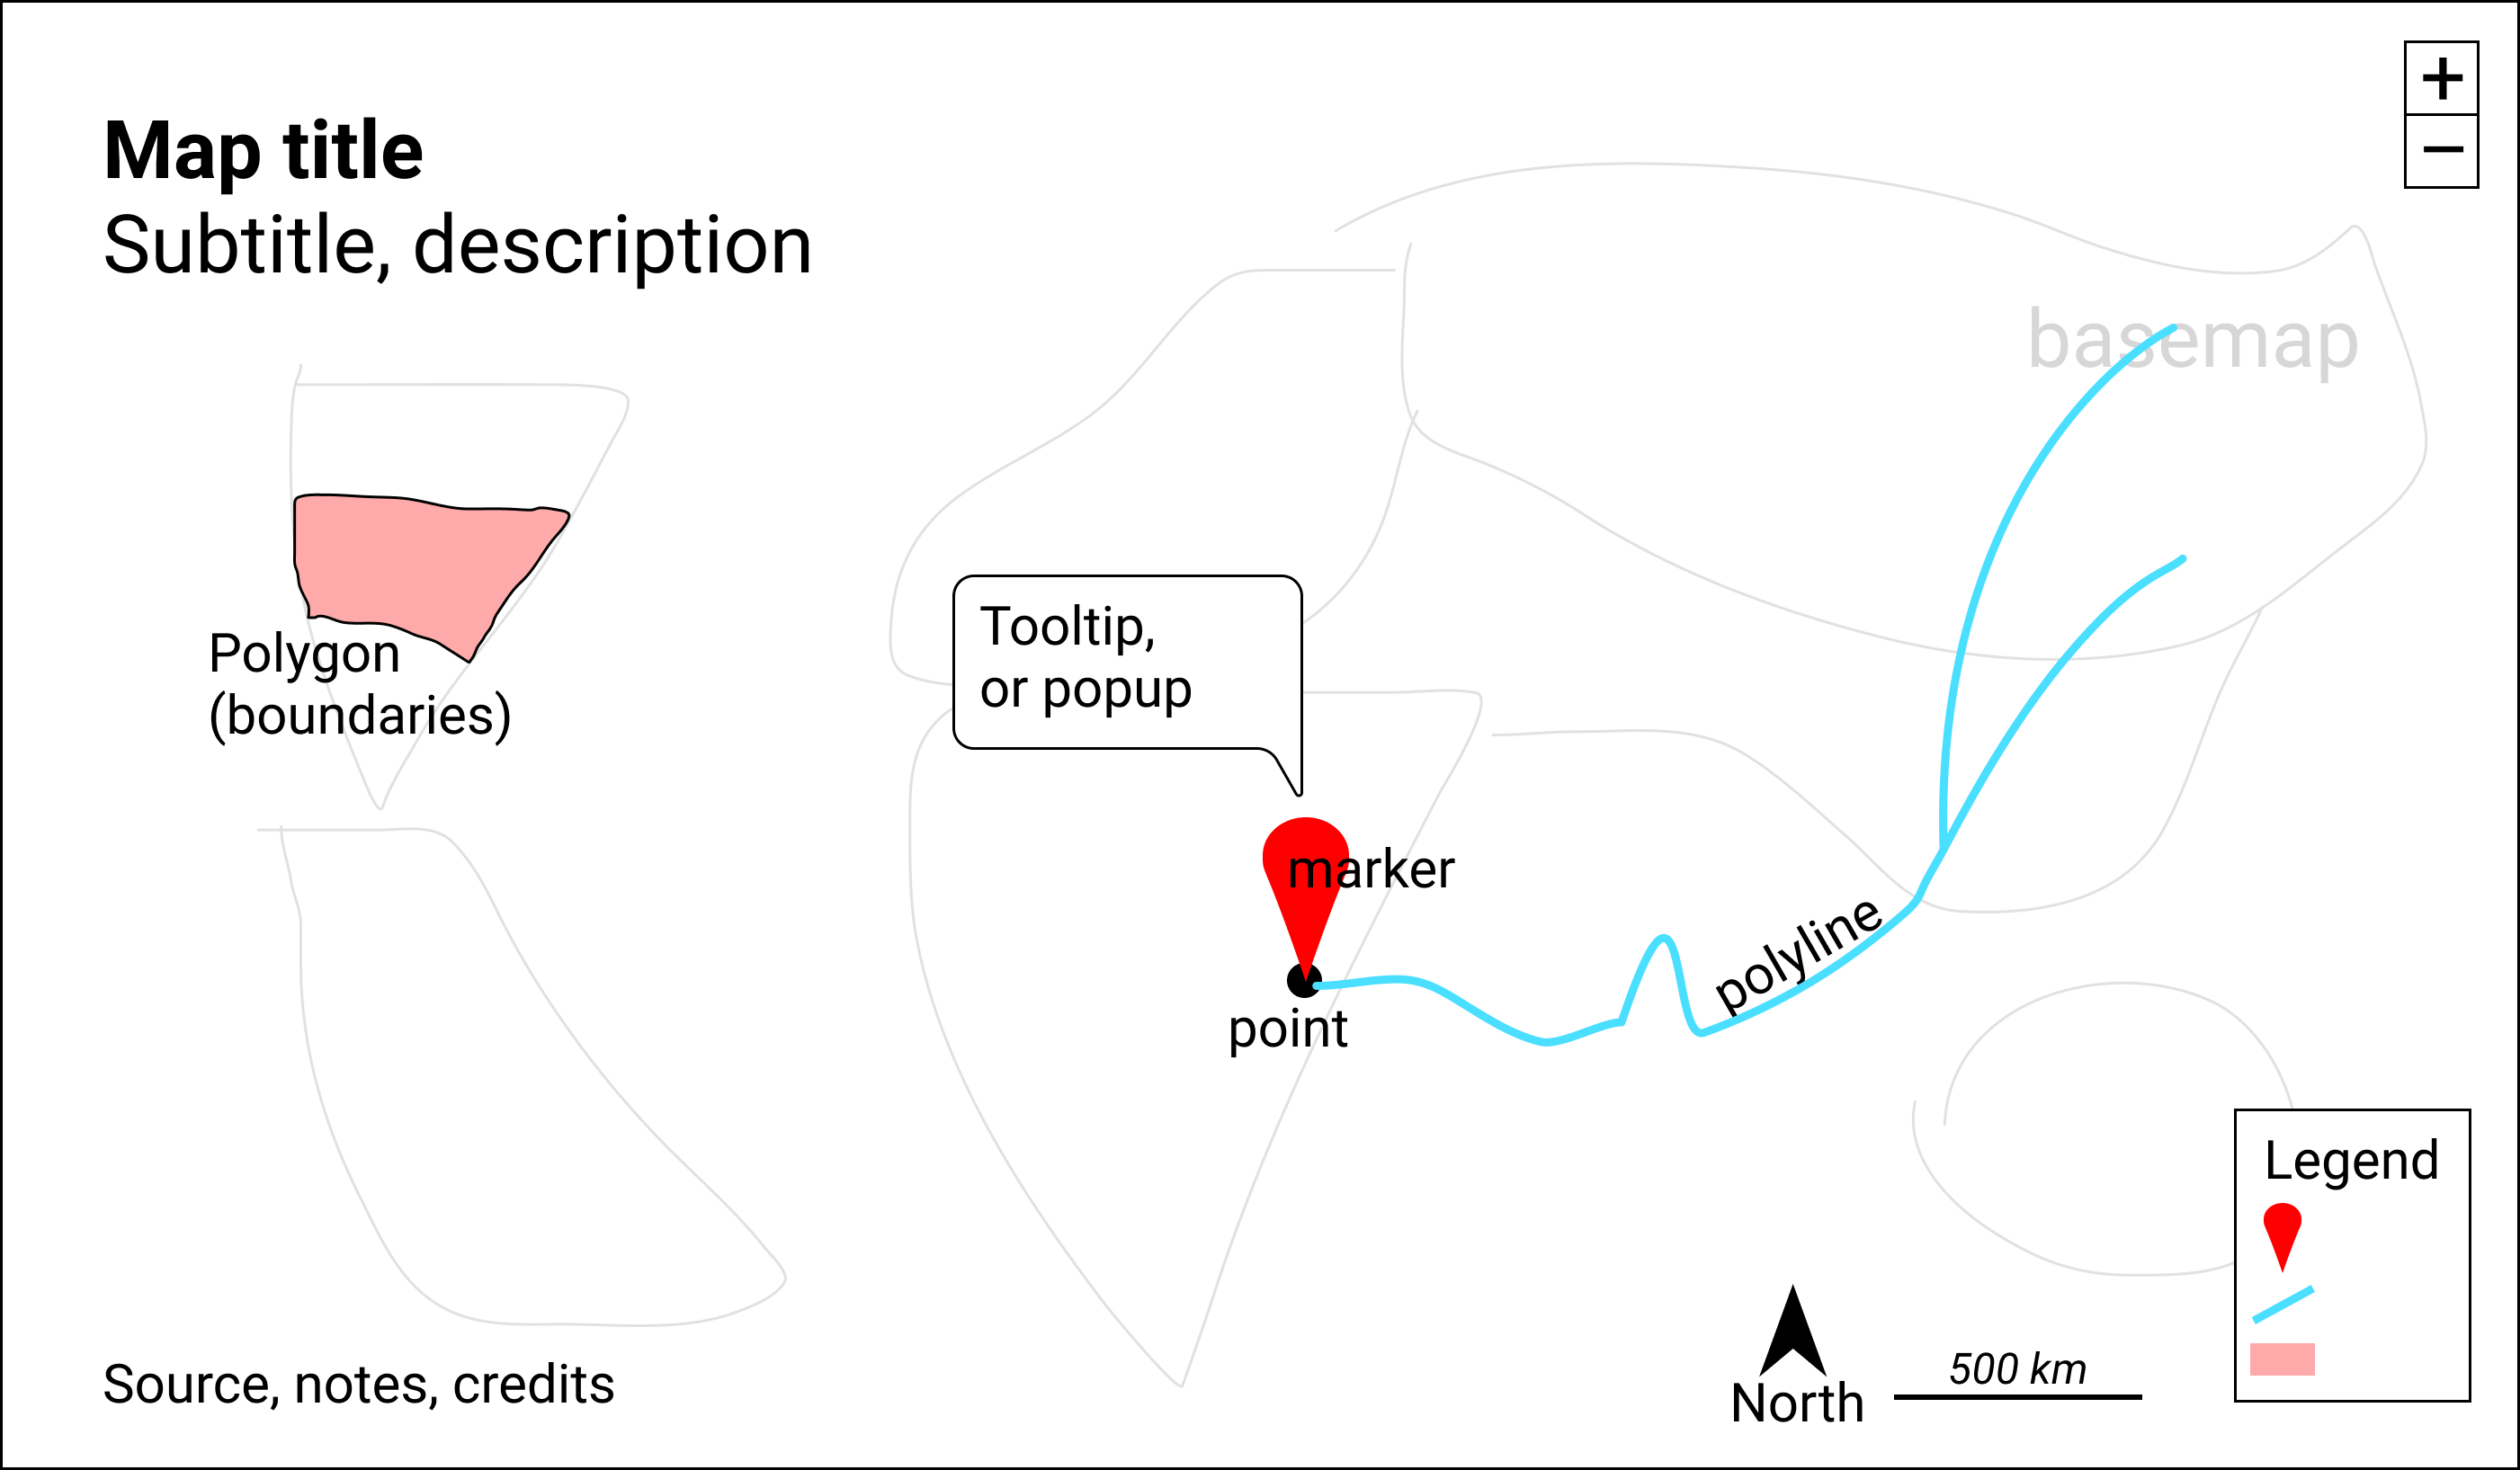
\includegraphics[width=\linewidth,height=0.58\textheight,keepaspectratio]{images/fig_7_2_map_elements.png}\\[0.12cm]
\figcaption{Các thành phần của bản đồ tương tác}
\end{column}
\end{columns}
\note{Bản đồ nền cung cấp bối cảnh; lớp dữ liệu phủ lên trên cho biết đối tượng đang nghiên cứu. Raster lưu thông tin theo ô ảnh, có thể là ảnh vệ tinh. Vector mô tả hình học bằng tọa độ nên giữ nét khi phóng gần; mức chi tiết vẫn phụ thuộc dữ liệu và cách dựng. Điểm có thể là Tượng Nữ thần Tự do tại vĩ độ 40.69, kinh độ -74.04. Tuyến là chuỗi điểm, vùng là ranh giới khép kín. Tiêu đề, chú giải, bối cảnh và nguồn giúp người đọc hiểu bản đồ. Nút zoom, tooltip và popup thường gặp ở bản đồ tương tác; mũi tên Bắc và thước tỷ lệ thêm khi cần, không phải mọi bản đồ đều bắt buộc. Nguồn: \url{https://handsondataviz.org/map-design.html}.}
\slidenumber{03}
\end{frame}

% ==================== SLIDE 4 ====================
\begin{frame}[plain,t]
\slideheader{Chương 7 • Map Your Data}{Chọn Kiểu Bản Đồ Theo Dữ Liệu}
\begin{columns}[T,onlytextwidth]
\begin{column}{0.30\textwidth}
\briefdef{Điểm}{→ Vị trí cụ thể}
\briefdef{Ký hiệu tỷ lệ}{→ Giá trị tại vị trí}
\briefdef{Phân vùng màu}{→ Giá trị theo vùng\\(choropleth)}
\vspace{0.20cm}
{\bodytext Công viên có thể là \textbf{điểm hoặc vùng}, tùy câu hỏi.\par}
\end{column}
\begin{column}{0.66\textwidth}\centering
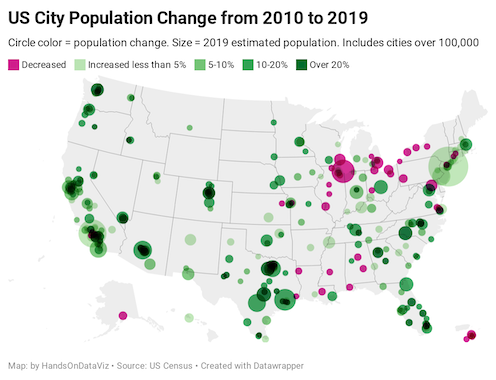
\includegraphics[width=\linewidth,height=0.56\textheight,keepaspectratio]{images/fig_7_34_symbol_map.png}\\[0.12cm]
\figcaption{Màu: biến động dân số • Kích thước: dân số 2019.}
\end{column}
\end{columns}
\note{Chọn kiểu bản đồ theo đại lượng cần thể hiện. Hình minh họa các thành phố Mỹ trên 100 nghìn dân: màu cho biết biến động dân số 2010--2019; kích thước ký hiệu biểu diễn dân số ước tính năm 2019. Điểm đánh dấu vị trí. Ký hiệu tỷ lệ có kích thước thay đổi theo giá trị tại vị trí. Choropleth tô màu vùng theo giá trị. Cùng một địa điểm có thể dùng nhiều cách biểu diễn: công viên là điểm khi cần tìm đường, là vùng khi cần tính diện tích đất công. Có thể dùng tâm điểm thành phố để vẽ vòng tròn, hoặc gộp số giường của từng bệnh viện theo hạt. Các loại khác gồm bản đồ nhiệt để thấy điểm nóng, bản đồ câu chuyện cho hành trình và đa tuyến cho mạng lưới. Nguồn: \url{https://handsondataviz.org/map.html} và \url{https://handsondataviz.org/map-design.html}.}
\slidenumber{04}
\end{frame}

% ==================== SLIDE 5 ====================
\begin{frame}[plain,t]
\slideheader{Chương 7 • Map Your Data}{Hai Biến: Cân Nhắc Biểu Đồ Phân Tán}
{\bodytext\textbf{Thu nhập:} tô màu\qquad\textbf{Học vấn:} kích thước ký hiệu\par}
\vspace{0.15cm}
\centering
% Show panels (c) and (d); crop only the two introductory single-variable panels.
% Original PNG is 563 x 599 pixels at 96 dpi; top trim = 285px * 72/96.
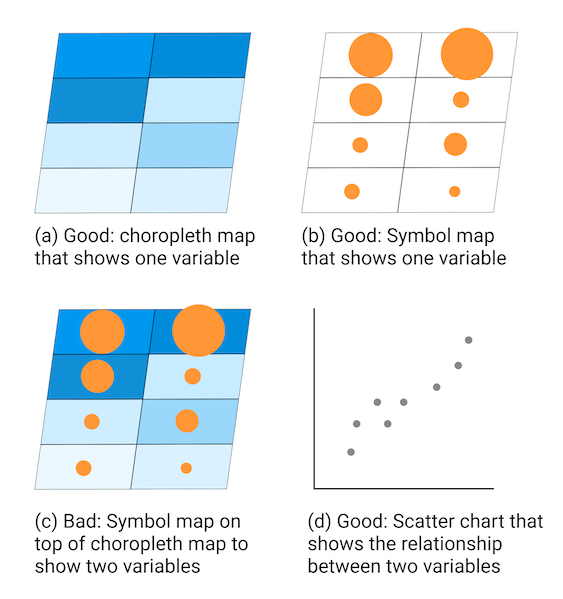
\includegraphics[width=0.88\linewidth,height=0.47\textheight,keepaspectratio,trim=0 0 0 213.75bp,clip]{images/fig_7_3_one_var_not_two.png}\\[0.10cm]
\begin{columns}[T,onlytextwidth]
\begin{column}{0.48\textwidth}{\bodytext\textbf{Chồng hai biến}\\[0.08cm]Khó nhận ra quan hệ\par}\end{column}
\begin{column}{0.48\textwidth}{\bodytext\textbf{Biểu đồ phân tán}\\[0.08cm]Quan hệ hai biến rõ hơn\par}\end{column}
\end{columns}
\takeaway{Có thể đặt bản đồ một biến cạnh biểu đồ phân tán.}
\note{Hình minh họa thu nhập và tỷ lệ có bằng đại học tại tám hạt. Bản đồ tô màu và ký hiệu tỷ lệ có thể đọc riêng, nhưng chồng hai cách mã hóa sẽ tăng công sức giải mã. Sách thường khuyên tránh cách chồng này và dùng biểu đồ phân tán nếu mục tiêu là tìm quan hệ. Đây là lời khuyên tránh chồng bản đồ ký hiệu lên choropleth, không phải lệnh cấm mọi cách mã hóa hai biến. Ví dụ bản đồ ký hiệu ở slide 4 vẫn có thể dùng cả màu lẫn kích thước của cùng ký hiệu. Có thể đặt một bản đồ cạnh biểu đồ phân tán để giữ cả bối cảnh không gian lẫn quan hệ số liệu. Nguồn: \url{https://handsondataviz.org/map-design.html}.}
\slidenumber{05}
\end{frame}

% ==================== SLIDE 6 ====================
\begin{frame}[plain,t]
\slideheader{Chương 7 • Map Your Data}{Chọn Mức Địa Lý Phù Hợp}
{\bodytext\textbf{MAUP:} Cách chia đơn vị không gian ảnh hưởng mẫu hình nhìn thấy.\par}
\vspace{0.12cm}
\centering
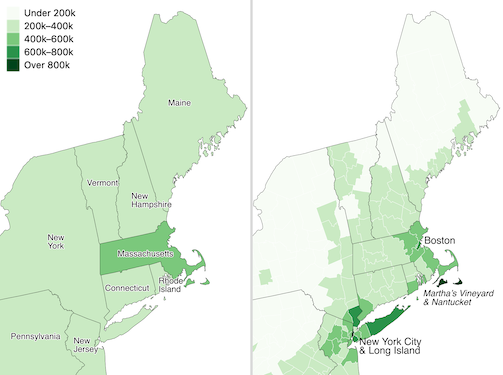
\includegraphics[width=0.88\linewidth,height=0.50\textheight,keepaspectratio]{images/fig_7_4_state_vs_county.png}\\[0.08cm]
\figcaption{Giá nhà điển hình, Đông Bắc Mỹ • 9/2020}
\vspace{0.12cm}
\begin{columns}[T,onlytextwidth]
\begin{column}{0.48\textwidth}{\bodytext\textbf{Cấp bang:} khác biệt giữa các bang\par}\end{column}
\begin{column}{0.48\textwidth}{\bodytext\textbf{Cấp hạt:} khác biệt trong mỗi bang\par}\end{column}
\end{columns}
\takeaway{Nhỏ hơn thường cho thêm chi tiết; quá chi tiết cũng che khuất mẫu hình.}
\note{MAUP là ảnh hưởng của cách chia hoặc gộp đơn vị không gian đến mẫu hình nhìn thấy. Hình dùng giá nhà điển hình Zillow tháng 9/2020; hai bản đồ dùng cùng thang màu và đều trung thực. Cấp bang phù hợp so sánh giữa các bang. Cấp hạt cho thấy các cụm giá nhà quanh New York, Long Island và Boston trong cùng bang. Đơn vị nhỏ hơn thường bộc lộ thêm chi tiết, nhưng chi tiết quá mức cũng có thể làm khó nhận ra mẫu hình. Nguồn: \url{https://handsondataviz.org/map-design.html}.}
\slidenumber{06}
\end{frame}

% ==================== SLIDE 7 ====================
\begin{frame}[plain,t]
\slideheader{Chương 7 • Map Your Data}{Chọn Bảng Màu Khớp Dữ Liệu}
\vspace{0.25cm}
\centering
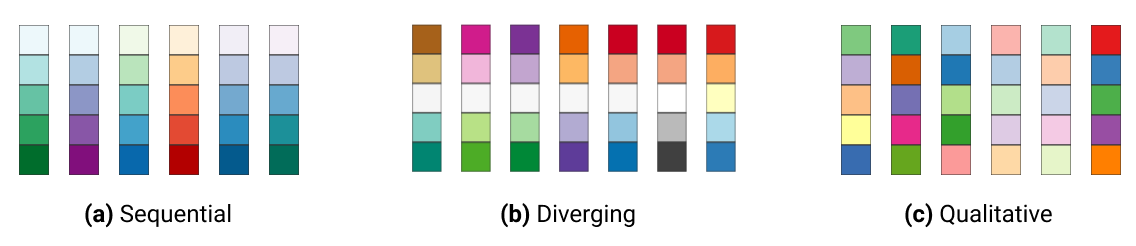
\includegraphics[width=0.96\linewidth,height=0.26\textheight,keepaspectratio]{images/fig_7_6_color_palettes.png}\\[0.25cm]
\begin{columns}[T,onlytextwidth]
\begin{column}{0.31\textwidth}\centering
{\fontsize{12pt}{15pt}\selectfont\bfseries Tuần tự}\\[0.12cm]
{\fontsize{9.5pt}{12.5pt}\selectfont\raggedright
\textbf{Dữ liệu số:} thấp $\rightarrow$ cao.\\[0.10cm]
Màu thường từ nhạt đến đậm.\\[0.10cm]
\textbf{Ví dụ:} thu nhập, lượng mưa.\par}
\end{column}
\begin{column}{0.31\textwidth}\centering
{\fontsize{12pt}{15pt}\selectfont\bfseries Phân kỳ}\\[0.12cm]
{\fontsize{9.5pt}{12.5pt}\selectfont\raggedright
\textbf{Trên / dưới một mốc:} 0, trung bình hoặc trung vị.\\[0.10cm]
Hai màu ở hai phía, màu trung tính ở giữa.\\[0.10cm]
\textbf{Ví dụ:} thu nhập so với trung bình.\par}
\end{column}
\begin{column}{0.31\textwidth}\centering
{\fontsize{12pt}{15pt}\selectfont\bfseries Định tính}\\[0.12cm]
{\fontsize{9.5pt}{12.5pt}\selectfont\raggedright
\textbf{Dữ liệu danh mục:} không xếp từ thấp đến cao.\\[0.10cm]
Mỗi loại dùng màu phân biệt.\\[0.10cm]
\textbf{Ví dụ:} đất ở, đất thương mại, mặt nước.\par}
\end{column}
\end{columns}
\note{Bảng màu phải khớp với dữ liệu và câu chuyện. Tuần tự phù hợp trật tự thấp tới cao. Phân kỳ có một mốc ở giữa để phân biệt hai phía. Định tính phân biệt danh mục mà không ngụ ý thứ tự. Cùng số liệu thu nhập bình quân đầu người Mỹ năm 2018, hai bảng màu nhấn hai cách đọc khác nhau. ColorBrewer hỗ trợ chọn bảng màu và kiểm tra khả năng đọc với người mù màu. Không phải mọi thiết kế đều bắt buộc mức cao mang màu đậm hơn. Nguồn: \url{https://handsondataviz.org/design-choropleth.html}.}
\slidenumber{07}
\end{frame}

% ==================== SLIDE 8 ====================
\begin{frame}[plain,t]
\slideheader{Chương 7 • Map Your Data}{Bậc Thang Hay Liên Tục?}
\begin{columns}[T,onlytextwidth]
\begin{column}{0.48\textwidth}
\briefdef{Bậc thang:}{nhóm màu rời rạc.}
\vspace{0.20cm}

\begin{tikzpicture}[x=0.9cm,y=0.6cm]
\foreach \i/\c in {0/10,1/30,2/50,3/75,4/100}{\fill[navyMain!\c!bgBeige] (\i,0) rectangle +(1,1);}
\end{tikzpicture}\par
\vspace{0.22cm}
{\bodytext\textbf{Làm rõ ngưỡng}\\[0.15cm]Ví dụ: vùng ngập khi nước biển dâng 1~m.\par}
\end{column}
\begin{column}{0.48\textwidth}
\briefdef{Liên tục:}{chuyển màu dần theo giá trị.}
\vspace{0.20cm}

\begin{tikzpicture}[x=0.9cm,y=0.6cm]\shade[left color=bgBeige,right color=navyMain] (0,0) rectangle (5,1);\end{tikzpicture}\par
\vspace{0.22cm}
{\bodytext\textbf{Thấy khác biệt tinh tế}\\[0.15cm]Giá trị gần nhau có màu gần nhau.\par}
\end{column}
\end{columns}
\vspace{0.35cm}
\figcaption{Minh họa khái niệm theo sách}
\takeaway{Cách chia khoảng màu ảnh hưởng đến những khác biệt người xem nhận ra.}
\note{Bậc thang chia giá trị thành những nhóm màu riêng để làm rõ ngưỡng. Ví dụ câu hỏi nơi nào ngập khi nước biển dâng một mét cần phân biệt trên và dưới ngưỡng. Liên tục cho thấy khác biệt tinh tế hơn, tránh tạo cảm giác hai giá trị rất gần nhau thuộc hai nhóm hoàn toàn khác nhau. Thử số nhóm phù hợp; nhiều nhóm hơn không tự động tốt hơn. Hai thang màu trên slide là minh họa khái niệm do người trình bày dựng theo sách, không phải hình gốc của sách. Nguồn: \url{https://handsondataviz.org/design-choropleth.html}. Tham khảo khi được hỏi về phương pháp chia màu: Xem histogram trước để hiểu phân bố. Tuyến tính đặt các khoảng giá trị đều trên thang màu; không nên nhầm với yêu cầu dữ liệu phải có phân bố chuẩn. Phân vị tạo các nhóm có số đơn vị gần bằng nhau, hữu ích khi dữ liệu lệch và cần phân biệt các mức ở giữa; giá trị trùng nhau có thể khiến nhóm không bằng hẳn. Jenks gom các giá trị gần nhau và là một phương án thỏa hiệp, không phải giải pháp hoàn hảo cho mọi dữ liệu. Thử các cách và tận dụng dải màu, không tự chọn ngưỡng để ép câu chuyện theo ý muốn. Nguồn: \url{https://handsondataviz.org/design-choropleth.html}.}
\slidenumber{08}
\end{frame}

% ==================== SLIDE 9 ====================
\begin{frame}[plain,t]
\slideheader{Chương 7 • Map Your Data}{Chuẩn Hóa Để So Sánh Có Ý Nghĩa}
{\bodytext\textbf{Chuẩn hóa:} đưa dữ liệu về thang chung để so sánh.\par}
\vspace{0.12cm}
\centering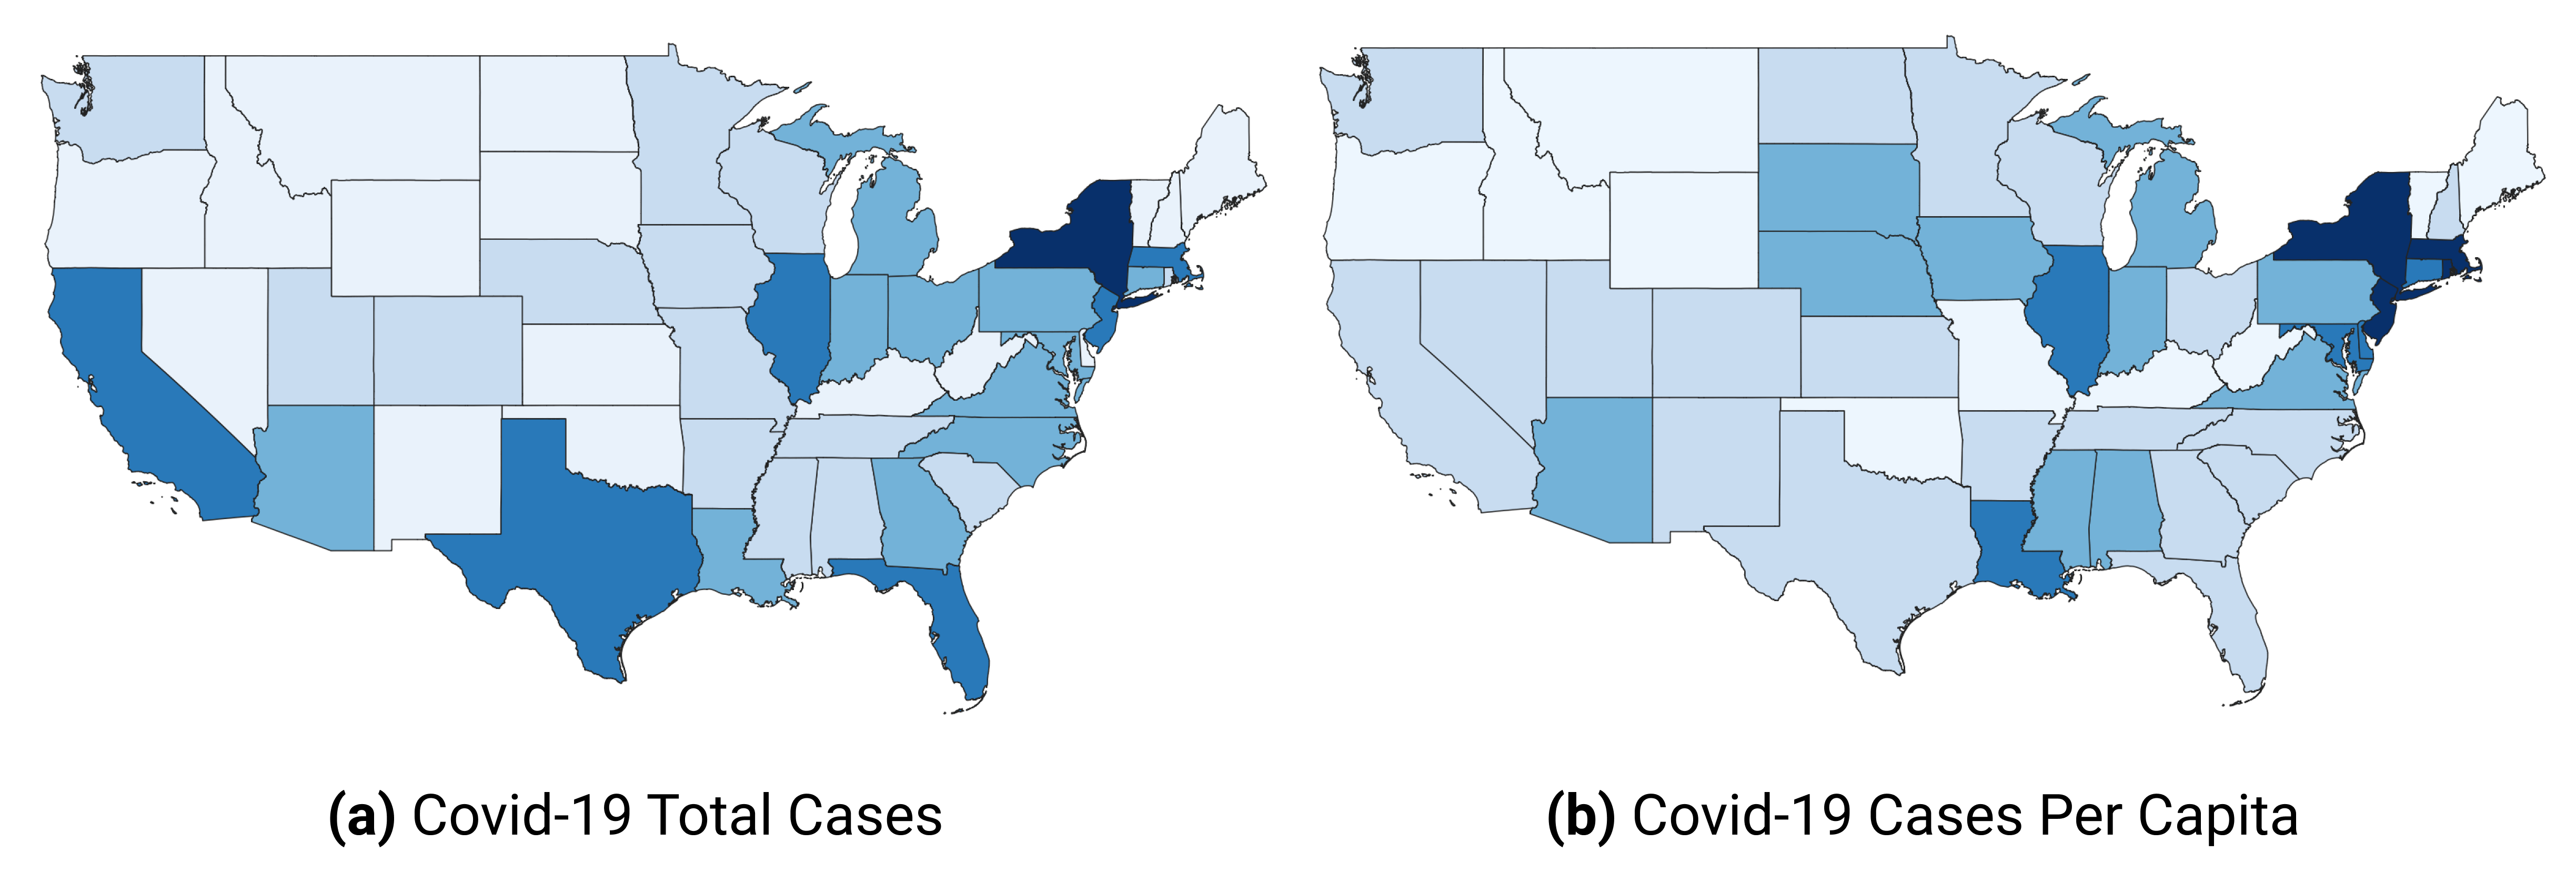
\includegraphics[width=0.95\linewidth,height=0.46\textheight,keepaspectratio]{images/fig_7_14_normalize_covid_map.png}\\[0.08cm]
\figcaption{Covid-19 tại Mỹ • 26/6/2020}
\vspace{0.16cm}
\begin{columns}[T,onlytextwidth]
\begin{column}{0.48\textwidth}{\bodytext\textbf{Tổng số ca ghi nhận}\\Số đếm → Quy mô\par}\end{column}
\begin{column}{0.48\textwidth}{\bodytext\textbf{Số ca theo dân số}\\Theo đầu người → Mức tương đối\par}\end{column}
\end{columns}
\takeaway{Choropleth thường phù hợp với tỷ lệ hoặc giá trị tương đối.}
\note{Chuẩn hóa giúp so sánh trên cùng một cơ sở. Tổng số ca ghi nhận mô tả quy mô; số ca chia dân số mô tả mức tương đối. Đây là ví dụ lịch sử từ New York Times ngày 26/6/2020, không phản ánh rủi ro hiện tại. California, Texas và Florida đông dân nên nổi bật trên bản đồ số ca. Khi chia dân số, các bang như New York, New Jersey và Massachusetts nổi bật hơn. Không gọi số đếm là sai trong mọi mục tiêu, và không suy luận rằng tỷ lệ ca ghi nhận đo toàn bộ nguy cơ hay số ca chưa phát hiện. Nguồn: \url{https://handsondataviz.org/normalize-choropleth.html}.}
\slidenumber{09}
\end{frame}

% ==================== SLIDE 10 ====================
\begin{frame}[plain,t]
\slideheader{Chương 7 • Map Your Data}{Bản Đồ Cập Nhật Vẫn Cần Kiểm Tra}
{\bodytext\textbf{Bản đồ cập nhật:} lấy dữ liệu mới từ nguồn được kết nối.\par}
\vspace{0.18cm}
\begin{columns}[c,onlytextwidth]
\begin{column}{0.30\textwidth}
\briefdef{Thời gian}{365 ngày}
\briefdef{Mức nghiêm trọng}{Vụ có người tử vong}
\briefdef{Tọa độ}{Loại điểm ngoài New York, như (0,0)}
\end{column}
\begin{column}{0.66\textwidth}\centering
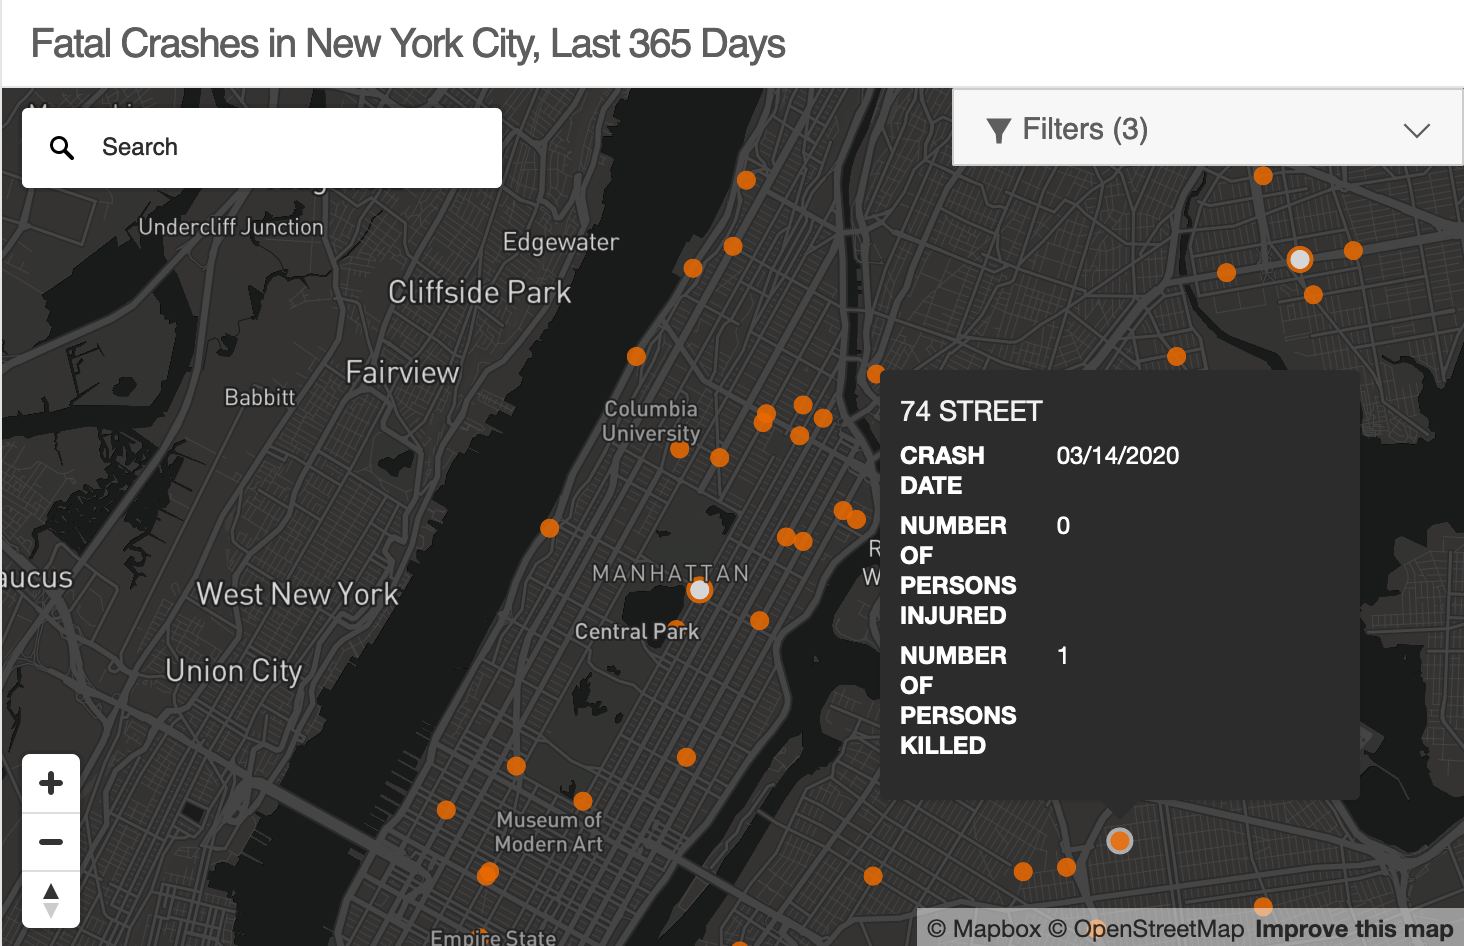
\includegraphics[width=\linewidth,height=0.52\textheight,keepaspectratio]{images/fig_7_61_nyc_crashes.png}\\[0.10cm]
\figcaption{Bản đồ tai nạn có người tử vong ở New York}
\end{column}
\end{columns}
\takeaway{Đúng dữ liệu • Đúng cách so sánh • Đúng câu chuyện}
\note{Bản đồ lấy dữ liệu từ nguồn được kết nối chỉ cập nhật khi nguồn và hệ thống vẫn được duy trì. Trong ví dụ tai nạn New York, lọc số người tử vong lớn hơn không, ngày tai nạn trong 365 ngày gần nhất và loại điểm ngoài phạm vi. Tọa độ (0,0) có thật trên Trái Đất nhưng nằm ngoài New York; trong dữ liệu tai nạn này nó có thể phản ánh lỗi hoặc thiếu vị trí. Điều kiện LATITUDE lớn hơn không chỉ là bộ lọc của trường hợp này, không phải phép kiểm tra tọa độ phổ quát. Đổi tên cột, thay nền tảng, ngắt API hoặc dừng cập nhật nguồn đều có thể làm bản đồ hỏng. Hình trong kho có số thứ tự khác phiên bản web, nên slide dùng chú thích mô tả. Kết lại: đúng dữ liệu, đúng cách so sánh và đúng câu chuyện. Nguồn: \url{https://handsondataviz.org/map-socrata.html}.}
\slidenumber{10}
\end{frame}

% ==================== BẮT ĐẦU PHẦN 4 ====================
% ==================== SLIDE 1 ====================
\begin{frame}[plain, c]


\begin{tikzpicture}[remember picture,overlay]
    \node[anchor=north west] at ($(current page.north west)+(1.0cm, -0.8cm)$) {
        \textcolor{navyMuted}{\fontsize{8.5pt}{10.5pt}\selectfont Tháng 10, 2026}
    };
    \node[anchor=west, text width=0.96\textwidth] at ($(current page.west)+(1.0cm, 0.3cm)$) {
        {\fontsize{13pt}{15pt}\selectfont \textbf{\color{navyMuted} PHẦN 4 • BÁO CÁO CHUYÊN ĐỀ}}\\[0.25cm]
        {\fontsize{28pt}{32pt}\selectfont \textbf{\color{navyMain} ĐẠO ĐỨC DỮ LIỆU \&}}\\[0.12cm]
        {\fontsize{20pt}{24pt}\selectfont \textbf{\color{navyMain} NGHỆ THUẬT KỂ CHUYỆN}}\\[0.35cm]
        {\fontsize{10pt}{13pt}\selectfont Chương 14 \& 15\\[0.15cm] Nhận diện gây hiểu lầm • Giảm thiên lệch • Kể chuyện dữ liệu}
    };
\end{tikzpicture}
\slidenumber{01}
\end{frame}

% ==================== SLIDE 2 ====================
\begin{frame}[plain,t]
\slideheader{01 • Nhận Diện Gây Hiểu Lầm}{Sai, Gây Hiểu Lầm Hay Trung Thực?}
\vspace{0.35cm}
\begin{columns}[T,onlytextwidth]
\begin{column}{0.315\textwidth}
\conceptcard{1. Sai (Wrong)}{Sai số liệu hoặc vi phạm nguyên tắc biểu diễn.}{\textbf{Ví dụ:} Biểu đồ cột cắt gốc 0; các phần của biểu đồ tròn không cộng thành 100\%.}
\end{column}
\begin{column}{0.315\textwidth}
\conceptcard{2. Gây hiểu lầm}{Số liệu đúng nhưng thang đo hoặc khung hình làm lệch cảm nhận.}{\textbf{Ví dụ:} Kéo rộng biểu đồ đường để xu hướng trông phẳng hơn.}
\end{column}
\begin{column}{0.315\textwidth}
\conceptcard{3. Trung thực}{Dữ liệu chính xác; cách biểu diễn phù hợp và ghi nhãn rõ.}{Cùng dữ liệu có thể có \textbf{nhiều cách nhìn trung thực}.}
\end{column}
\end{columns}
\slidenumber{02}
\end{frame}

% ==================== SLIDE 3 ====================
\begin{frame}[plain, t]
\slideheader{01 • Nhận Diện Gây Hiểu Lầm}{Thang Đo \& Khung Hình Làm Lệch Cảm Nhận}
\begin{columns}[T,onlytextwidth]
\begin{column}{0.50\textwidth}
{\fontsize{9.5pt}{12.8pt}\selectfont
\textbf{1. Cắt trục tung của biểu đồ cột}
\begin{itemize}\setlength{\itemsep}{3pt}
\item GDP Mỹ chỉ tăng \textbf{0,96\%} (quý II--III/2019). Cắt bỏ mốc 0 khiến mức tăng nhỏ trông lớn hơn nhiều.
\item Trục tung cần bắt đầu từ \textbf{0} để chiều cao cột phản ánh đúng giá trị.
\end{itemize}
\vspace{0.12cm}
\textbf{2. Kéo bẹt biểu đồ đường}
\begin{itemize}\setlength{\itemsep}{3pt}
\item Kéo biểu đồ rộng ra làm đường trông phẳng hơn, dù dữ liệu không đổi.
\item Đọc \textbf{giá trị và mốc thời gian trên trục} để biết tăng bao nhiêu, trong bao lâu; đừng chỉ nhìn độ dốc.
\end{itemize}
}
\end{column}
\begin{column}{0.46\textwidth}
\centering
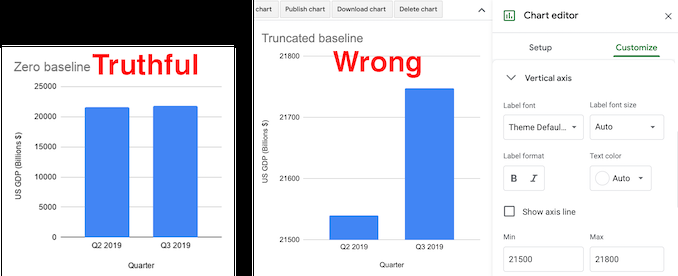
\includegraphics[width=\textwidth, height=0.31\textheight, keepaspectratio]{images/fig_14_1_truncated_gdp.png}\\[0.08cm]
{\fontsize{7pt}{9pt}\selectfont\textcolor{navyMuted}{\textit{Hình 14.1: Cắt trục phóng đại mức tăng GDP.}}}\\[0.18cm]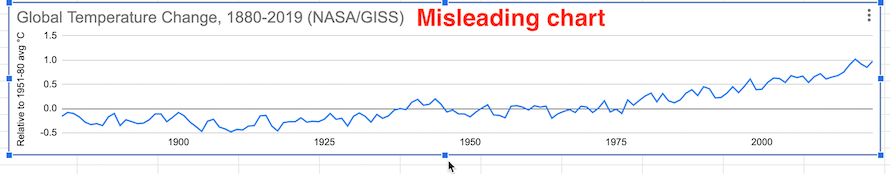
\includegraphics[width=\textwidth, height=0.23\textheight, keepaspectratio]{images/fig_14_4_aspect_ratio_stretched.png}\\[0.08cm]
{\fontsize{7pt}{9pt}\selectfont\textcolor{navyMuted}{\textit{Hình 14.4: Kéo rộng khung hình làm đường trông phẳng hơn.}}}
\end{column}
\end{columns}
\slidenumber{03}
\end{frame}

% ==================== SLIDE 4 ====================
\begin{frame}[plain,t]
\slideheader{01 • Nhận Diện Gây Hiểu Lầm}{Một Bộ Dữ Liệu, Nhiều Cách Diễn Giải Đúng}
{\fontsize{8.5pt}{11pt}\selectfont
\textbf{Tỷ trọng thu nhập quốc dân trước thuế của nhóm 1\% có thu nhập cao nhất:}\\
Mỹ \textbf{20,5\%} (2018); Brazil \textbf{28,3\%} (2015).
}
\vspace{0.15cm}
\begin{columns}[T,onlytextwidth]
\begin{column}{0.48\textwidth}
{\fontsize{9.5pt}{12pt}\selectfont\textbf{1. Thang màu liên tục}}\\[0.08cm]
\centering
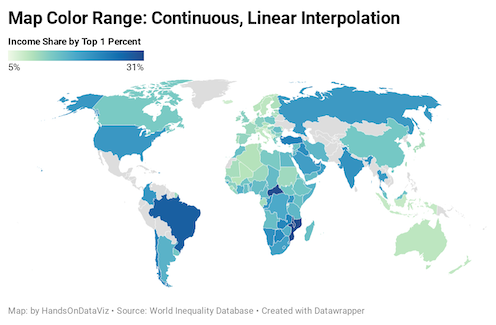
\includegraphics[width=\linewidth,height=0.215\textheight,keepaspectratio]{images/fig_14_12_inequality_continuous.png}\\[0.06cm]
{\fontsize{7pt}{9pt}\selectfont\color{navyMuted}Hình 14.12}\\[0.02cm]
\raggedright
{\fontsize{9pt}{11.5pt}\selectfont Mỹ có \textbf{màu trung bình} trên thang 5\%--31\%.}
\end{column}
\begin{column}{0.48\textwidth}
{\fontsize{9.5pt}{12pt}\selectfont\textbf{2. Chia ba nhóm theo Jenks}}\\[0.08cm]
\centering
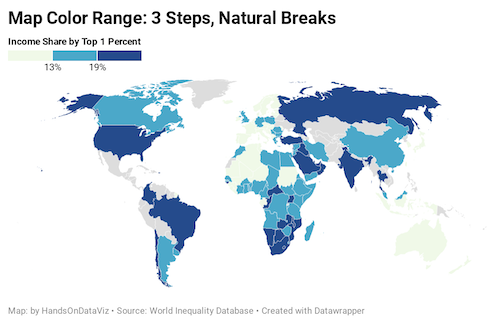
\includegraphics[width=\linewidth,height=0.215\textheight,keepaspectratio]{images/fig_14_13_inequality_jenks.png}\\[0.06cm]
{\fontsize{7pt}{9pt}\selectfont\color{navyMuted}Hình 14.13}\\[0.02cm]
\raggedright
{\fontsize{9pt}{11.5pt}\selectfont Mỹ thuộc \textbf{nhóm màu đậm nhất} (từ 19\%), cùng Brazil.}
\end{column}
\end{columns}
\vspace{0.05cm}
\begin{columns}[c,onlytextwidth]
\begin{column}{0.34\textwidth}\centering
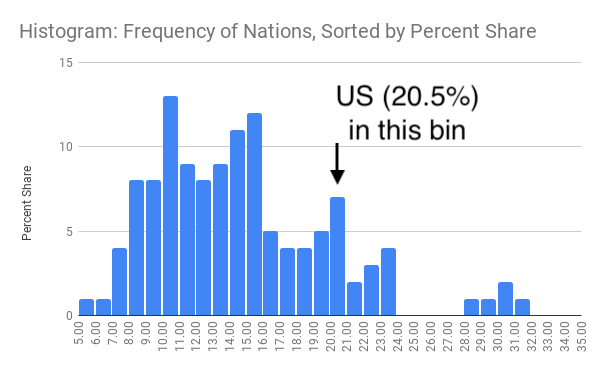
\includegraphics[width=\linewidth,height=0.16\textheight,keepaspectratio]{images/fig_14_14_inequality_histogram.png}\\[0.04cm]
{\fontsize{7pt}{9pt}\selectfont\color{navyMuted}Hình 14.14 • Phân bố các quốc gia}
\end{column}
\begin{column}{0.62\textwidth}
{\fontsize{9pt}{11.5pt}\selectfont
\textbf{Vì sao Mỹ đổi màu?}\\[0.08cm]
Histogram giúp hiểu cách chia nhóm. Số liệu của Mỹ vẫn là \textbf{20,5\%}. \textbf{Cần xem thang màu để hiểu đúng bản đồ.}
}
\end{column}
\end{columns}
\slidenumber{04}
\end{frame}

% ==================== SLIDE 5 ====================
\begin{frame}[plain,t]
\slideheader{02 • Giảm Thiên Lệch}{Thiên Lệch Khi Thu Thập Và Đọc Dữ Liệu}
\vspace{0.20cm}
\begin{columns}[T,onlytextwidth]
\begin{column}{0.48\textwidth}
\begin{tikzpicture}
\node[fill=boxBg,draw=navyMain,line width=0.7pt,rounded corners=4pt,
inner sep=9pt,align=left] {\parbox[t][5.5cm][t]{\dimexpr\linewidth-20pt\relax}{\raggedright
{\fontsize{11pt}{14pt}\selectfont\bfseries 1. Thiên lệch chọn mẫu}\\[0.18cm]
{\fontsize{9pt}{12pt}\selectfont Cách thu thập làm mẫu không đại diện và kết quả lệch đi.}\\[0.14cm]
{\fontsize{9pt}{12pt}\selectfont \textbf{Ví dụ:} Đo chiều cao người vừa tập bóng rổ, rồi suy rộng cho mọi người.}\\[0.15cm]
{\centering
\begin{tikzpicture}[>=Stealth]
\node[draw=navyMain,fill=bgBeige,rounded corners=3pt,text width=3.7cm,align=center,inner sep=5pt,font=\fontsize{10pt}{12pt}\selectfont] (sample) {\textbf{Người vừa tập bóng rổ}};
\node[draw=navyMain,fill=bgBeige,rounded corners=3pt,text width=3.7cm,align=center,inner sep=5pt,font=\fontsize{10pt}{12pt}\selectfont,below=0.65cm of sample] (population) {\textbf{Toàn bộ dân số}};
\draw[->,accentRed,line width=1pt] (sample.south) -- (population.north)
node[midway,fill=boxBg,text=accentRed,inner sep=2pt,font=\fontsize{8.5pt}{10pt}\selectfont] {Không thể suy rộng};
\end{tikzpicture}
\par}
\vspace{0.05cm}
{\fontsize{9pt}{12pt}\selectfont\color{navyMain}Kiểm tra tính đại diện của mẫu.}
}};
\end{tikzpicture}
\end{column}
\begin{column}{0.48\textwidth}
\begin{tikzpicture}
\node[fill=boxBg,draw=navyMain,line width=0.7pt,rounded corners=4pt,
inner sep=9pt,align=left] {\parbox[t][5.5cm][t]{\dimexpr\linewidth-20pt\relax}{\raggedright
{\fontsize{11pt}{14pt}\selectfont\bfseries 2. Thiên lệch nhận thức}\\[0.18cm]
{\fontsize{9pt}{12pt}\selectfont Cách suy nghĩ của con người làm lệch cách hiểu dữ liệu.}\\[0.14cm]
{\fontsize{9pt}{12pt}\selectfont \textbf{Ví dụ:} hiệu ứng đóng khung}\\[0.25cm]
{\centering
\begin{tikzpicture}
\node[align=center,text=accentRed] at (0,0) {{\fontsize{30pt}{34pt}\selectfont\bfseries 5\%}\\[0.10cm]{\fontsize{10pt}{12pt}\selectfont tử vong}};
\node[align=center,text=navyMain] at (3.16,0) {{\fontsize{30pt}{34pt}\selectfont\bfseries 95\%}\\[0.10cm]{\fontsize{10pt}{12pt}\selectfont sống sót}};
\node[font=\fontsize{11pt}{13pt}\selectfont,text=navyMuted] at (1.55,0.10) {$\longleftrightarrow$};
\end{tikzpicture}
\par}
\vspace{0.10cm}
{\fontsize{10pt}{13pt}\selectfont\color{navyMain}\bfseries Cùng số liệu, khác cảm nhận.}
}};
\end{tikzpicture}
\end{column}
\end{columns}
\slidenumber{05}
\end{frame}

% ==================== SLIDE 6 ====================
\begin{frame}[plain,t]
\slideheader{02 • Giảm Thiên Lệch}{Thiên Lệch Thuật Toán Và Giữa Các Nhóm}
\begin{columns}[c,onlytextwidth]
\begin{column}{0.30\textwidth}
{\fontsize{11pt}{14pt}\selectfont\bfseries 3. Thuật toán}\\[0.12cm]
{\fontsize{10pt}{13pt}\selectfont Ưu tiên kết quả \textbf{có hệ thống}}\\[0.10cm]
{\fontsize{9pt}{12pt}\selectfont\color{navyMuted}ProPublica • Dự báo tái phạm}
\end{column}
\begin{column}{0.66\textwidth}
\begin{tikzpicture}
\node[fill=boxBg,draw=navyMain,rounded corners=4pt,inner sep=8pt,
text width=\dimexpr\linewidth-18pt\relax,align=left] {
{\fontsize{10pt}{13pt}\selectfont\bfseries Tỷ lệ dự báo sai: gần gấp đôi}\\[0.08cm]
{\fontsize{9pt}{12pt}\selectfont Bị cáo da đen so với bị cáo da trắng}\\[0.08cm]
{\fontsize{8.5pt}{11pt}\selectfont\color{navyMuted}Sai số dự báo $\neq$ tỷ lệ tái phạm thực}
};
\end{tikzpicture}
\end{column}
\end{columns}
\vspace{0.28cm}
{\color{navyMuted!35}\hrule height 0.4pt}
\vspace{0.30cm}
\begin{columns}[c,onlytextwidth]
\begin{column}{0.30\textwidth}
{\fontsize{11pt}{14pt}\selectfont\bfseries 4. Giữa các nhóm}\\[0.12cm]
{\fontsize{10pt}{13pt}\selectfont
\textbf{Ưu ái / phân biệt đối xử}\\
Chủng tộc • Giới • $\ldots$
\begin{itemize}\setlength{\itemsep}{3pt}
\item Thứ tự: White / Men
\item Nhóm bị bỏ sót?
\item Mốc so sánh?
\end{itemize}
}
\end{column}
\begin{column}{0.32\textwidth}\centering
\parbox[c][3.25cm][c]{\linewidth}{\centering
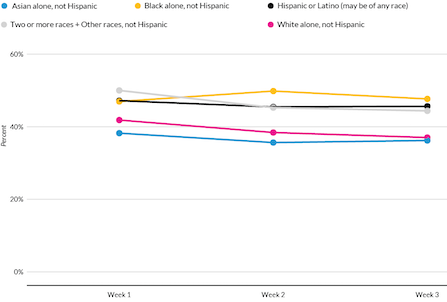
\includegraphics[width=\linewidth,height=3.25cm,keepaspectratio]{images/fig_14_15_deficit_chart.png}}\\[0.10cm]
{\fontsize{8pt}{10pt}\selectfont\color{navyMuted}Hình 14.15 • Gộp nhóm\\\phantom{+ mốc tham chiếu}}
\end{column}
\begin{column}{0.32\textwidth}\centering
\parbox[c][3.25cm][c]{\linewidth}{\centering
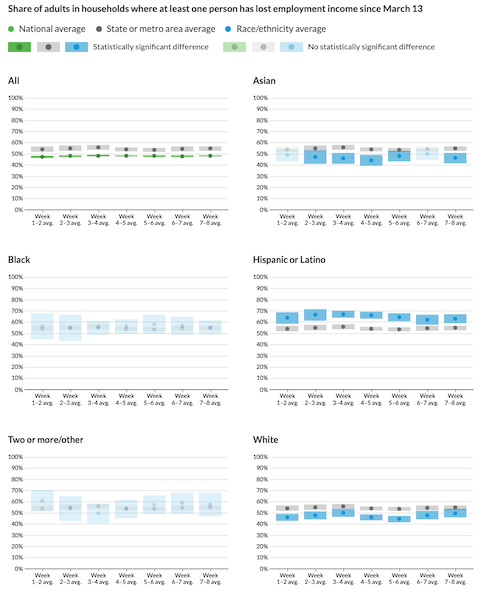
\includegraphics[width=\linewidth,height=3.25cm,keepaspectratio]{images/fig_14_16_separate_panels.png}}\\[0.10cm]
{\fontsize{8pt}{10pt}\selectfont\color{navyMuted}Hình 14.16 • Tách nhóm\\+ mốc tham chiếu}
\end{column}
\end{columns}
\note{Thuật toán: sách dẫn điều tra ProPublica về tỷ lệ dự báo sai bị cáo da đen sẽ tái phạm gần gấp đôi bị cáo da trắng. Đây là sai số dự báo, không phải tỷ lệ tái phạm thực tế. Giữa các nhóm: cách sắp thứ tự, bỏ sót nhóm và chọn mốc so sánh có thể củng cố định kiến. Hình 14.15 và 14.16 minh họa cách gộp hoặc tách nhóm trong dữ liệu mất thu nhập việc làm. Schwabish và Feng đề xuất tách nhóm; Dougherty và Ilyankou chưa bị thuyết phục rằng cách này tất yếu tăng công bằng, vì có thể khó nhận ra rào cản cấu trúc.}
\slidenumber{06}
\end{frame}

% ==================== SLIDE 7 ====================
\begin{frame}[plain, t]
\slideheader{02 • Giảm Thiên Lệch}{Bản Đồ Có Thể Làm Ai Bị Lu Mờ?}
\begin{columns}[T,onlytextwidth]
\begin{column}{0.50\textwidth}
{\fontsize{9.5pt}{12.8pt}\selectfont
\textbf{Diện tích không đồng nghĩa với dân số}
\begin{itemize}\setlength{\itemsep}{3pt}
\item Vùng đất rộng dễ thu hút chú ý dù có ít dân.
\item \textbf{Cartogram} điều chỉnh diện tích theo dân số hoặc số phiếu đại cử tri, tùy đại lượng cần so sánh.
\end{itemize}
\vspace{0.15cm}
\textbf{Kiểm tra những nơi bị bỏ sót}
\begin{itemize}\setlength{\itemsep}{3pt}
\item Bản đồ chỉ có 50 bang có thể bỏ qua Washington D.C. và các lãnh thổ của Mỹ.
\item Chọn phạm vi bao quát đúng các cộng đồng thuộc câu hỏi nghiên cứu.
\end{itemize}
}
\end{column}
\begin{column}{0.46\textwidth}
\centering
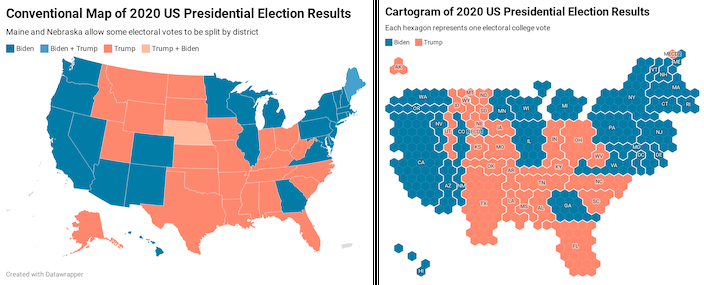
\includegraphics[width=\textwidth, height=0.31\textheight, keepaspectratio]{images/fig_14_17_cartogram_election.png}\\[0.08cm]
{\fontsize{7pt}{9pt}\selectfont\textcolor{navyMuted}{\textit{Hình 14.17: Cartogram biểu diễn số phiếu đại cử tri.}}}\\[0.12cm]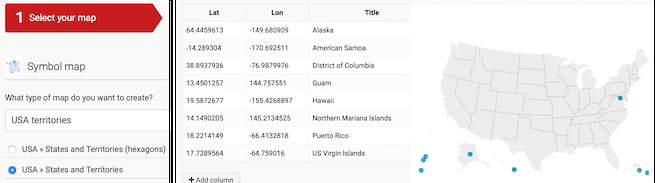
\includegraphics[width=\textwidth, height=0.28\textheight, keepaspectratio]{images/fig_14_19_map_exclusion.png}\\[0.08cm]
{\fontsize{7pt}{9pt}\selectfont\textcolor{navyMuted}{\textit{Hình 14.19: Hiển thị cả D.C. và các lãnh thổ.}}}
\end{column}
\end{columns}
\slidenumber{07}
\end{frame}

% ==================== SLIDE 8 ====================
\begin{frame}[plain,t]
\slideheader{03 • Kể Chuyện Dữ Liệu}{Kể Chuyện Theo Tell -- Show -- Why}
{\fontsize{10pt}{13pt}\selectfont Biểu đồ cần người dẫn giải: nêu \textbf{xu hướng chung} và chọn vài \textbf{điểm nổi bật} làm minh chứng.}
\vspace{0.4cm}
\begin{columns}[T,onlytextwidth]
\begin{column}{0.315\textwidth}
\conceptcard{1. TELL}{\textbf{Nêu phát hiện}}{Viết thông điệp chính thành một câu tiêu đề ngắn.}
\end{column}
\begin{column}{0.315\textwidth}
\conceptcard{2. SHOW}{\textbf{Đưa bằng chứng}}{Dùng biểu đồ hoặc bản đồ trung thực để hỗ trợ thông điệp.}
\end{column}
\begin{column}{0.315\textwidth}
\conceptcard{3. WHY}{\textbf{Giải thích ý nghĩa}}{Nêu phát hiện giúp người xem hiểu vấn đề hoặc cân nhắc hành động nào.}
\end{column}
\end{columns}
\slidenumber{08}
\end{frame}

% ==================== SLIDE 9 ====================
\begin{frame}[plain, t]
\slideheader{03 • Kể Chuyện Dữ Liệu}{Từ Câu Hỏi Đến Câu Chuyện Dữ Liệu}
\begin{columns}[T,onlytextwidth]
\begin{column}{0.50\textwidth}
{\fontsize{9.5pt}{12.8pt}\selectfont
\begin{enumerate}\setlength{\itemsep}{7pt}
\item \textbf{Vấn đề:} Vì sao chủ đề này đáng quan tâm?
\item \textbf{Câu hỏi:} Cần tìm câu trả lời cụ thể nào?
\item \textbf{Dữ liệu:} Nguồn nào giúp trả lời câu hỏi?
\item \textbf{Trực quan hóa:} Biểu đồ nào làm rõ phát hiện?
\end{enumerate}
\vspace{0.18cm}
\calloutbox[\textwidth]{Kiểm tra mạch kể}{Nêu vấn đề trước khi đưa đáp án. Kết luận cuối cùng phải trả lời đúng câu hỏi ban đầu.}
}
\end{column}
\begin{column}{0.46\textwidth}
\centering
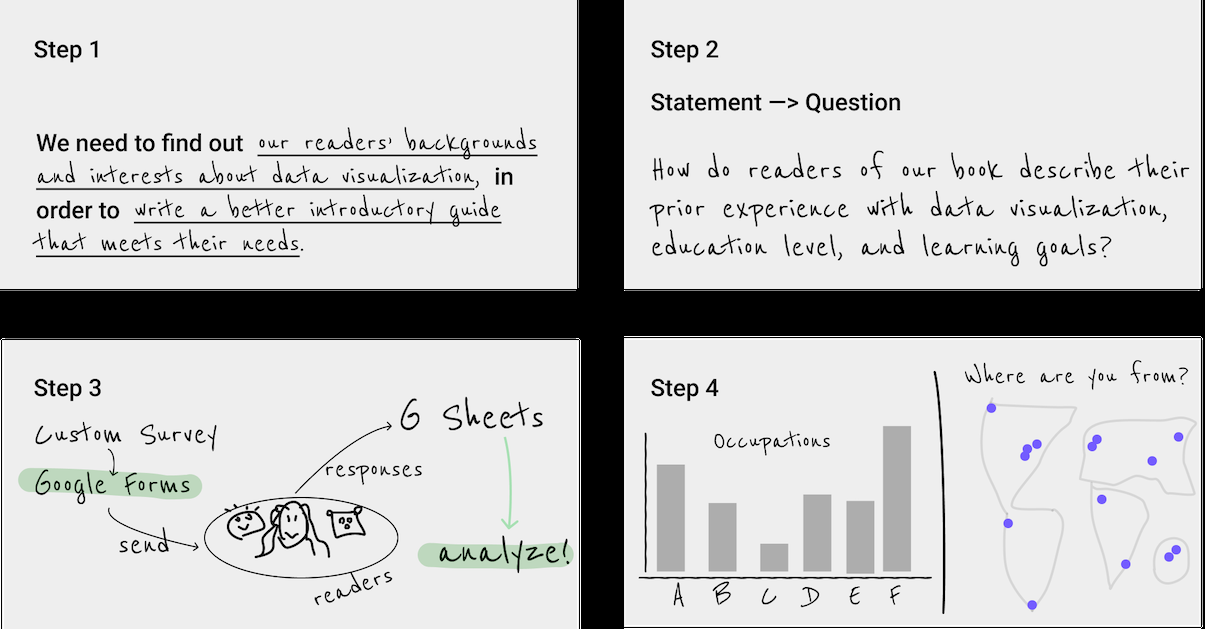
\includegraphics[width=\textwidth, height=0.49\textheight, keepaspectratio]{images/fig_15_1_storyboard_sketch.png}\\[0.08cm]
{\fontsize{7pt}{9pt}\selectfont\textcolor{navyMuted}{\textit{Hình 15.1: Phác thảo storyboard trước khi thiết kế.}}}
\end{column}
\end{columns}
\slidenumber{09}
\end{frame}

% ==================== SLIDE 10 ====================
\begin{frame}[plain,t]
\slideheader{03 • Kể Chuyện Dữ Liệu}{Màu Sắc \& Chú Thích Làm Rõ Thông Điệp}
{\fontsize{10pt}{13pt}\selectfont
\textbf{Sản lượng nhựa toàn cầu, 1950--2015:} hơn một nửa lượng nhựa trong dữ liệu được sản xuất từ năm 2000.
\\[0.12cm]
Đổi sang biểu đồ miền, tô đậm giai đoạn này và ghi chú trực tiếp để làm rõ phát hiện.
}
\vspace{0.25cm}
\begin{columns}[T,onlytextwidth]
\begin{column}{0.475\textwidth}\centering
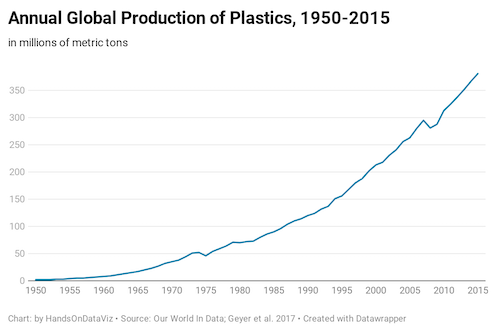
\includegraphics[width=\linewidth,height=0.39\textheight,keepaspectratio]{images/fig_15_3_plastics_line.png}\\[0.12cm]
{\fontsize{7.5pt}{9.5pt}\selectfont\color{navyMuted}Hình 15.3 • Biểu đồ đường ban đầu}
\end{column}
\begin{column}{0.495\textwidth}\centering
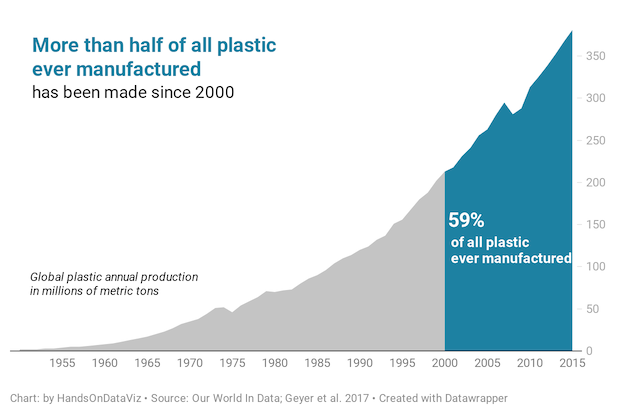
\includegraphics[width=\linewidth,height=0.39\textheight,keepaspectratio]{images/fig_15_5_plastics_annotated.png}\\[0.12cm]
{\fontsize{7.5pt}{9.5pt}\selectfont\color{navyMuted}Hình 15.5 • Tô màu và chú thích phát hiện}
\end{column}
\end{columns}
\slidenumber{10}
\end{frame}

% ==================== SLIDE 11 ====================
\begin{frame}[plain, t]
\slideheader{Phần 4 • Tổng Kết}{Kể Chuyện Thuyết Phục \& Có Trách Nhiệm}
\begin{columns}[T,onlytextwidth]
\begin{column}{0.50\textwidth}
{\fontsize{9.5pt}{12.8pt}\selectfont
\begin{itemize}\setlength{\itemsep}{6pt}
\item \textbf{Trung thực:} Chọn thang đo phù hợp; kết luận trong giới hạn bằng chứng.
\item \textbf{Minh bạch:} Ghi nguồn, cách xử lý dữ liệu và những hạn chế.
\item \textbf{Thừa nhận bất định:} Phân biệt số liệu quan sát với dự báo; ghi rõ giả định và mức độ chắc chắn.
\end{itemize}
\vspace{0.15cm}
\calloutbox[\textwidth]{Thông điệp phần 4}{Kiểm tra cách biểu diễn, nhận diện thiên lệch và dùng Tell -- Show -- Why để dẫn dắt câu chuyện.}
\vspace{0.18cm}
{\color{navyMuted}\textbf{Cảm ơn \& Hỏi đáp}}
}
\end{column}
\begin{column}{0.46\textwidth}
\centering
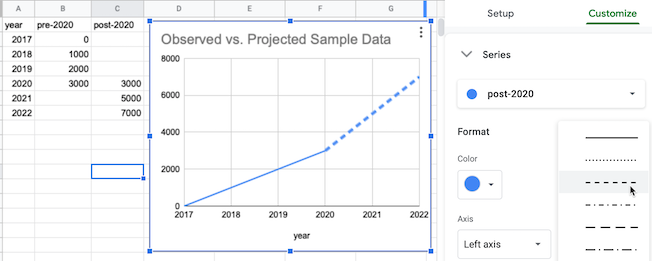
\includegraphics[width=\textwidth, height=0.47\textheight, keepaspectratio,trim=112.5bp 7.5bp 161.25bp 15bp,clip]{images/fig_15_6_observed_vs_projected.png}\\[0.08cm]
{\fontsize{7pt}{9pt}\selectfont\textcolor{navyMuted}{\textit{Hình 15.6: Nét liền cho quan sát, nét đứt cho dự báo.}}}
\end{column}
\end{columns}
\slidenumber{11}
\end{frame}

\end{document}